%File: anonymous-submission-latex-2024.tex
\documentclass[letterpaper]{article} % DO NOT CHANGE THIS
\usepackage{aaai24}  % DO NOT CHANGE THIS
\usepackage{times}  % DO NOT CHANGE THIS
\usepackage{helvet}  % DO NOT CHANGE THIS
\usepackage{courier}  % DO NOT CHANGE THIS
\usepackage[hyphens]{url}  % DO NOT CHANGE THIS
\usepackage{graphicx} % DO NOT CHANGE THIS
\urlstyle{rm} % DO NOT CHANGE THIS
\def\UrlFont{\rm}  % DO NOT CHANGE THIS
\usepackage{natbib}  % DO NOT CHANGE THIS AND DO NOT ADD ANY OPTIONS TO IT
\usepackage{caption} % DO NOT CHANGE THIS AND DO NOT ADD ANY OPTIONS TO IT
\frenchspacing  % DO NOT CHANGE THIS
\setlength{\pdfpagewidth}{8.5in} % DO NOT CHANGE THIS
\setlength{\pdfpageheight}{11in} % DO NOT CHANGE THIS
\usepackage{algorithm}
\usepackage{algorithmic}
\usepackage{multirow}
\usepackage{enumitem, array}
%%%%% NEW MATH DEFINITIONS %%%%%

\usepackage{amsmath,bm}

% Mark sections of captions for referring to divisions of figures
\newcommand{\figleft}{{\em (Left)}}
\newcommand{\figcenter}{{\em (Center)}}
\newcommand{\figright}{{\em (Right)}}
\newcommand{\figtop}{{\em (Top)}}
\newcommand{\figbottom}{{\em (Bottom)}}
\newcommand{\captiona}{{\em (a)}}
\newcommand{\captionb}{{\em (b)}}
\newcommand{\captionc}{{\em (c)}}
\newcommand{\captiond}{{\em (d)}}

% Highlight a newly defined term
\newcommand{\newterm}[1]{{\bf #1}}


% Figure reference, lower-case.
\def\figref#1{figure~\ref{#1}}
% Figure reference, capital. For start of sentence
\def\Figref#1{Figure~\ref{#1}}
\def\twofigref#1#2{figures \ref{#1} and \ref{#2}}
\def\quadfigref#1#2#3#4{figures \ref{#1}, \ref{#2}, \ref{#3} and \ref{#4}}
% Section reference, lower-case.
\def\secref#1{section~\ref{#1}}
% Section reference, capital.
\def\Secref#1{Section~\ref{#1}}
% Reference to two sections.
\def\twosecrefs#1#2{sections \ref{#1} and \ref{#2}}
% Reference to three sections.
\def\secrefs#1#2#3{sections \ref{#1}, \ref{#2} and \ref{#3}}
% Reference to an equation, lower-case.
\def\eqref#1{equation~\ref{#1}}
% Reference to an equation, upper case
\def\Eqref#1{Equation~\ref{#1}}
% A raw reference to an equation---avoid using if possible
\def\plaineqref#1{\ref{#1}}
% Reference to a chapter, lower-case.
\def\chapref#1{chapter~\ref{#1}}
% Reference to an equation, upper case.
\def\Chapref#1{Chapter~\ref{#1}}
% Reference to a range of chapters
\def\rangechapref#1#2{chapters\ref{#1}--\ref{#2}}
% Reference to an algorithm, lower-case.
\def\algref#1{algorithm~\ref{#1}}
% Reference to an algorithm, upper case.
\def\Algref#1{Algorithm~\ref{#1}}
\def\twoalgref#1#2{algorithms \ref{#1} and \ref{#2}}
\def\Twoalgref#1#2{Algorithms \ref{#1} and \ref{#2}}
% Reference to a part, lower case
\def\partref#1{part~\ref{#1}}
% Reference to a part, upper case
\def\Partref#1{Part~\ref{#1}}
\def\twopartref#1#2{parts \ref{#1} and \ref{#2}}

\def\ceil#1{\lceil #1 \rceil}
\def\floor#1{\lfloor #1 \rfloor}
\def\1{\bm{1}}
\newcommand{\train}{\mathcal{D}}
\newcommand{\valid}{\mathcal{D_{\mathrm{valid}}}}
\newcommand{\test}{\mathcal{D_{\mathrm{test}}}}

\def\eps{{\epsilon}}


% Random variables
\def\reta{{\textnormal{$\eta$}}}
\def\ra{{\textnormal{a}}}
\def\rb{{\textnormal{b}}}
\def\rc{{\textnormal{c}}}
\def\rd{{\textnormal{d}}}
\def\re{{\textnormal{e}}}
\def\rf{{\textnormal{f}}}
\def\rg{{\textnormal{g}}}
\def\rh{{\textnormal{h}}}
\def\ri{{\textnormal{i}}}
\def\rj{{\textnormal{j}}}
\def\rk{{\textnormal{k}}}
\def\rl{{\textnormal{l}}}
% rm is already a command, just don't name any random variables m
\def\rn{{\textnormal{n}}}
\def\ro{{\textnormal{o}}}
\def\rp{{\textnormal{p}}}
\def\rq{{\textnormal{q}}}
\def\rr{{\textnormal{r}}}
\def\rs{{\textnormal{s}}}
\def\rt{{\textnormal{t}}}
\def\ru{{\textnormal{u}}}
\def\rv{{\textnormal{v}}}
\def\rw{{\textnormal{w}}}
\def\rx{{\textnormal{x}}}
\def\ry{{\textnormal{y}}}
\def\rz{{\textnormal{z}}}

% Random vectors
\def\rvepsilon{{\mathbf{\epsilon}}}
\def\rvtheta{{\mathbf{\theta}}}
\def\rva{{\mathbf{a}}}
\def\rvb{{\mathbf{b}}}
\def\rvc{{\mathbf{c}}}
\def\rvd{{\mathbf{d}}}
\def\rve{{\mathbf{e}}}
\def\rvf{{\mathbf{f}}}
\def\rvg{{\mathbf{g}}}
\def\rvh{{\mathbf{h}}}
\def\rvu{{\mathbf{i}}}
\def\rvj{{\mathbf{j}}}
\def\rvk{{\mathbf{k}}}
\def\rvl{{\mathbf{l}}}
\def\rvm{{\mathbf{m}}}
\def\rvn{{\mathbf{n}}}
\def\rvo{{\mathbf{o}}}
\def\rvp{{\mathbf{p}}}
\def\rvq{{\mathbf{q}}}
\def\rvr{{\mathbf{r}}}
\def\rvs{{\mathbf{s}}}
\def\rvt{{\mathbf{t}}}
\def\rvu{{\mathbf{u}}}
\def\rvv{{\mathbf{v}}}
\def\rvw{{\mathbf{w}}}
\def\rvx{{\mathbf{x}}}
\def\rvy{{\mathbf{y}}}
\def\rvz{{\mathbf{z}}}

% Elements of random vectors
\def\erva{{\textnormal{a}}}
\def\ervb{{\textnormal{b}}}
\def\ervc{{\textnormal{c}}}
\def\ervd{{\textnormal{d}}}
\def\erve{{\textnormal{e}}}
\def\ervf{{\textnormal{f}}}
\def\ervg{{\textnormal{g}}}
\def\ervh{{\textnormal{h}}}
\def\ervi{{\textnormal{i}}}
\def\ervj{{\textnormal{j}}}
\def\ervk{{\textnormal{k}}}
\def\ervl{{\textnormal{l}}}
\def\ervm{{\textnormal{m}}}
\def\ervn{{\textnormal{n}}}
\def\ervo{{\textnormal{o}}}
\def\ervp{{\textnormal{p}}}
\def\ervq{{\textnormal{q}}}
\def\ervr{{\textnormal{r}}}
\def\ervs{{\textnormal{s}}}
\def\ervt{{\textnormal{t}}}
\def\ervu{{\textnormal{u}}}
\def\ervv{{\textnormal{v}}}
\def\ervw{{\textnormal{w}}}
\def\ervx{{\textnormal{x}}}
\def\ervy{{\textnormal{y}}}
\def\ervz{{\textnormal{z}}}

% Random matrices
\def\rmA{{\mathbf{A}}}
\def\rmB{{\mathbf{B}}}
\def\rmC{{\mathbf{C}}}
\def\rmD{{\mathbf{D}}}
\def\rmE{{\mathbf{E}}}
\def\rmF{{\mathbf{F}}}
\def\rmG{{\mathbf{G}}}
\def\rmH{{\mathbf{H}}}
\def\rmI{{\mathbf{I}}}
\def\rmJ{{\mathbf{J}}}
\def\rmK{{\mathbf{K}}}
\def\rmL{{\mathbf{L}}}
\def\rmM{{\mathbf{M}}}
\def\rmN{{\mathbf{N}}}
\def\rmO{{\mathbf{O}}}
\def\rmP{{\mathbf{P}}}
\def\rmQ{{\mathbf{Q}}}
\def\rmR{{\mathbf{R}}}
\def\rmS{{\mathbf{S}}}
\def\rmT{{\mathbf{T}}}
\def\rmU{{\mathbf{U}}}
\def\rmV{{\mathbf{V}}}
\def\rmW{{\mathbf{W}}}
\def\rmX{{\mathbf{X}}}
\def\rmY{{\mathbf{Y}}}
\def\rmZ{{\mathbf{Z}}}

% Elements of random matrices
\def\ermA{{\textnormal{A}}}
\def\ermB{{\textnormal{B}}}
\def\ermC{{\textnormal{C}}}
\def\ermD{{\textnormal{D}}}
\def\ermE{{\textnormal{E}}}
\def\ermF{{\textnormal{F}}}
\def\ermG{{\textnormal{G}}}
\def\ermH{{\textnormal{H}}}
\def\ermI{{\textnormal{I}}}
\def\ermJ{{\textnormal{J}}}
\def\ermK{{\textnormal{K}}}
\def\ermL{{\textnormal{L}}}
\def\ermM{{\textnormal{M}}}
\def\ermN{{\textnormal{N}}}
\def\ermO{{\textnormal{O}}}
\def\ermP{{\textnormal{P}}}
\def\ermQ{{\textnormal{Q}}}
\def\ermR{{\textnormal{R}}}
\def\ermS{{\textnormal{S}}}
\def\ermT{{\textnormal{T}}}
\def\ermU{{\textnormal{U}}}
\def\ermV{{\textnormal{V}}}
\def\ermW{{\textnormal{W}}}
\def\ermX{{\textnormal{X}}}
\def\ermY{{\textnormal{Y}}}
\def\ermZ{{\textnormal{Z}}}

% Vectors
\def\vzero{{\bm{0}}}
\def\vone{{\bm{1}}}
\def\vmu{{\bm{\mu}}}
\def\vtheta{{\bm{\theta}}}
\def\va{{\bm{a}}}
\def\vb{{\bm{b}}}
\def\vc{{\bm{c}}}
\def\vd{{\bm{d}}}
\def\ve{{\bm{e}}}
\def\vf{{\bm{f}}}
\def\vg{{\bm{g}}}
\def\vh{{\bm{h}}}
\def\vi{{\bm{i}}}
\def\vj{{\bm{j}}}
\def\vk{{\bm{k}}}
\def\vl{{\bm{l}}}
\def\vm{{\bm{m}}}
\def\vn{{\bm{n}}}
\def\vo{{\bm{o}}}
\def\vp{{\bm{p}}}
\def\vq{{\bm{q}}}
\def\vr{{\bm{r}}}
\def\vs{{\bm{s}}}
\def\vt{{\bm{t}}}
\def\vu{{\bm{u}}}
\def\vv{{\bm{v}}}
\def\vw{{\bm{w}}}
\def\vx{{\bm{x}}}
\def\vy{{\bm{y}}}
\def\vz{{\bm{z}}}

% Elements of vectors
\def\evalpha{{\alpha}}
\def\evbeta{{\beta}}
\def\evepsilon{{\epsilon}}
\def\evlambda{{\lambda}}
\def\evomega{{\omega}}
\def\evmu{{\mu}}
\def\evpsi{{\psi}}
\def\evsigma{{\sigma}}
\def\evtheta{{\theta}}
\def\eva{{a}}
\def\evb{{b}}
\def\evc{{c}}
\def\evd{{d}}
\def\eve{{e}}
\def\evf{{f}}
\def\evg{{g}}
\def\evh{{h}}
\def\evi{{i}}
\def\evj{{j}}
\def\evk{{k}}
\def\evl{{l}}
\def\evm{{m}}
\def\evn{{n}}
\def\evo{{o}}
\def\evp{{p}}
\def\evq{{q}}
\def\evr{{r}}
\def\evs{{s}}
\def\evt{{t}}
\def\evu{{u}}
\def\evv{{v}}
\def\evw{{w}}
\def\evx{{x}}
\def\evy{{y}}
\def\evz{{z}}

% Matrix
\def\mA{{\bm{A}}}
\def\mB{{\bm{B}}}
\def\mC{{\bm{C}}}
\def\mD{{\bm{D}}}
\def\mE{{\bm{E}}}
\def\mF{{\bm{F}}}
\def\mG{{\bm{G}}}
\def\mH{{\bm{H}}}
\def\mI{{\bm{I}}}
\def\mJ{{\bm{J}}}
\def\mK{{\bm{K}}}
\def\mL{{\bm{L}}}
\def\mM{{\bm{M}}}
\def\mN{{\bm{N}}}
\def\mO{{\bm{O}}}
\def\mP{{\bm{P}}}
\def\mQ{{\bm{Q}}}
\def\mR{{\bm{R}}}
\def\mS{{\bm{S}}}
\def\mT{{\bm{T}}}
\def\mU{{\bm{U}}}
\def\mV{{\bm{V}}}
\def\mW{{\bm{W}}}
\def\mX{{\bm{X}}}
\def\mY{{\bm{Y}}}
\def\mZ{{\bm{Z}}}
\def\mBeta{{\bm{\beta}}}
\def\mPhi{{\bm{\Phi}}}
\def\mLambda{{\bm{\Lambda}}}
\def\mSigma{{\bm{\Sigma}}}

% Tensor
\DeclareMathAlphabet{\mathsfit}{\encodingdefault}{\sfdefault}{m}{sl}
\SetMathAlphabet{\mathsfit}{bold}{\encodingdefault}{\sfdefault}{bx}{n}
\newcommand{\tens}[1]{\bm{\mathsfit{#1}}}
\def\tA{{\tens{A}}}
\def\tB{{\tens{B}}}
\def\tC{{\tens{C}}}
\def\tD{{\tens{D}}}
\def\tE{{\tens{E}}}
\def\tF{{\tens{F}}}
\def\tG{{\tens{G}}}
\def\tH{{\tens{H}}}
\def\tI{{\tens{I}}}
\def\tJ{{\tens{J}}}
\def\tK{{\tens{K}}}
\def\tL{{\tens{L}}}
\def\tM{{\tens{M}}}
\def\tN{{\tens{N}}}
\def\tO{{\tens{O}}}
\def\tP{{\tens{P}}}
\def\tQ{{\tens{Q}}}
\def\tR{{\tens{R}}}
\def\tS{{\tens{S}}}
\def\tT{{\tens{T}}}
\def\tU{{\tens{U}}}
\def\tV{{\tens{V}}}
\def\tW{{\tens{W}}}
\def\tX{{\tens{X}}}
\def\tY{{\tens{Y}}}
\def\tZ{{\tens{Z}}}


% Graph
\def\gA{{\mathcal{A}}}
\def\gB{{\mathcal{B}}}
\def\gC{{\mathcal{C}}}
\def\gD{{\mathcal{D}}}
\def\gE{{\mathcal{E}}}
\def\gF{{\mathcal{F}}}
\def\gG{{\mathcal{G}}}
\def\gH{{\mathcal{H}}}
\def\gI{{\mathcal{I}}}
\def\gJ{{\mathcal{J}}}
\def\gK{{\mathcal{K}}}
\def\gL{{\mathcal{L}}}
\def\gM{{\mathcal{M}}}
\def\gN{{\mathcal{N}}}
\def\gO{{\mathcal{O}}}
\def\gP{{\mathcal{P}}}
\def\gQ{{\mathcal{Q}}}
\def\gR{{\mathcal{R}}}
\def\gS{{\mathcal{S}}}
\def\gT{{\mathcal{T}}}
\def\gU{{\mathcal{U}}}
\def\gV{{\mathcal{V}}}
\def\gW{{\mathcal{W}}}
\def\gX{{\mathcal{X}}}
\def\gY{{\mathcal{Y}}}
\def\gZ{{\mathcal{Z}}}

% Sets
\def\sA{{\mathbb{A}}}
\def\sB{{\mathbb{B}}}
\def\sC{{\mathbb{C}}}
\def\sD{{\mathbb{D}}}
% Don't use a set called E, because this would be the same as our symbol
% for expectation.
\def\sF{{\mathbb{F}}}
\def\sG{{\mathbb{G}}}
\def\sH{{\mathbb{H}}}
\def\sI{{\mathbb{I}}}
\def\sJ{{\mathbb{J}}}
\def\sK{{\mathbb{K}}}
\def\sL{{\mathbb{L}}}
\def\sM{{\mathbb{M}}}
\def\sN{{\mathbb{N}}}
\def\sO{{\mathbb{O}}}
\def\sP{{\mathbb{P}}}
\def\sQ{{\mathbb{Q}}}
\def\sR{{\mathbb{R}}}
\def\sS{{\mathbb{S}}}
\def\sT{{\mathbb{T}}}
\def\sU{{\mathbb{U}}}
\def\sV{{\mathbb{V}}}
\def\sW{{\mathbb{W}}}
\def\sX{{\mathbb{X}}}
\def\sY{{\mathbb{Y}}}
\def\sZ{{\mathbb{Z}}}

% Entries of a matrix
\def\emLambda{{\Lambda}}
\def\emA{{A}}
\def\emB{{B}}
\def\emC{{C}}
\def\emD{{D}}
\def\emE{{E}}
\def\emF{{F}}
\def\emG{{G}}
\def\emH{{H}}
\def\emI{{I}}
\def\emJ{{J}}
\def\emK{{K}}
\def\emL{{L}}
\def\emM{{M}}
\def\emN{{N}}
\def\emO{{O}}
\def\emP{{P}}
\def\emQ{{Q}}
\def\emR{{R}}
\def\emS{{S}}
\def\emT{{T}}
\def\emU{{U}}
\def\emV{{V}}
\def\emW{{W}}
\def\emX{{X}}
\def\emY{{Y}}
\def\emZ{{Z}}
\def\emSigma{{\Sigma}}

% entries of a tensor
% Same font as tensor, without \bm wrapper
\newcommand{\etens}[1]{\mathsfit{#1}}
\def\etLambda{{\etens{\Lambda}}}
\def\etA{{\etens{A}}}
\def\etB{{\etens{B}}}
\def\etC{{\etens{C}}}
\def\etD{{\etens{D}}}
\def\etE{{\etens{E}}}
\def\etF{{\etens{F}}}
\def\etG{{\etens{G}}}
\def\etH{{\etens{H}}}
\def\etI{{\etens{I}}}
\def\etJ{{\etens{J}}}
\def\etK{{\etens{K}}}
\def\etL{{\etens{L}}}
\def\etM{{\etens{M}}}
\def\etN{{\etens{N}}}
\def\etO{{\etens{O}}}
\def\etP{{\etens{P}}}
\def\etQ{{\etens{Q}}}
\def\etR{{\etens{R}}}
\def\etS{{\etens{S}}}
\def\etT{{\etens{T}}}
\def\etU{{\etens{U}}}
\def\etV{{\etens{V}}}
\def\etW{{\etens{W}}}
\def\etX{{\etens{X}}}
\def\etY{{\etens{Y}}}
\def\etZ{{\etens{Z}}}

% The true underlying data generating distribution
\newcommand{\pdata}{p_{\rm{data}}}
% The empirical distribution defined by the training set
\newcommand{\ptrain}{\hat{p}_{\rm{data}}}
\newcommand{\Ptrain}{\hat{P}_{\rm{data}}}
% The model distribution
\newcommand{\pmodel}{p_{\rm{model}}}
\newcommand{\Pmodel}{P_{\rm{model}}}
\newcommand{\ptildemodel}{\tilde{p}_{\rm{model}}}
% Stochastic autoencoder distributions
\newcommand{\pencode}{p_{\rm{encoder}}}
\newcommand{\pdecode}{p_{\rm{decoder}}}
\newcommand{\precons}{p_{\rm{reconstruct}}}

\newcommand{\laplace}{\mathrm{Laplace}} % Laplace distribution

\newcommand{\E}{\mathbb{E}}
\newcommand{\Ls}{\mathcal{L}}
\newcommand{\R}{\mathbb{R}}
\newcommand{\emp}{\tilde{p}}
\newcommand{\lr}{\alpha}
\newcommand{\reg}{\lambda}
\newcommand{\rect}{\mathrm{rectifier}}
\newcommand{\softmax}{\mathrm{softmax}}
\newcommand{\sigmoid}{\sigma}
\newcommand{\softplus}{\zeta}
\newcommand{\KL}{D_{\mathrm{KL}}}
\newcommand{\Var}{\mathrm{Var}}
\newcommand{\standarderror}{\mathrm{SE}}
\newcommand{\Cov}{\mathrm{Cov}}
% Wolfram Mathworld says $L^2$ is for function spaces and $\ell^2$ is for vectors
% But then they seem to use $L^2$ for vectors throughout the site, and so does
% wikipedia.
\newcommand{\normlzero}{L^0}
\newcommand{\normlone}{L^1}
\newcommand{\normltwo}{L^2}
\newcommand{\normlp}{L^p}
\newcommand{\normmax}{L^\infty}

\newcommand{\parents}{Pa} % See usage in notation.tex. Chosen to match Daphne's book.

\DeclareMathOperator*{\argmax}{arg\,max}
\DeclareMathOperator*{\argmin}{arg\,min}

\DeclareMathOperator{\sign}{sign}
\DeclareMathOperator{\Tr}{Tr}
\let\ab\allowbreak
\newcommand{\ols}[1]{\mskip.5\thinmuskip\overline{\mskip-.5\thinmuskip {#1} \mskip-.5\thinmuskip}\mskip.5\thinmuskip} % overline short
\newcommand{\olsi}[1]{\,\overline{\!{#1}}} % overline short italic
\makeatletter
\newcommand\closure[1]{
  \tctestifnum{\count@stringtoks{#1}>1} %checks if number of chars in arg > 1 (including '\')
  {\ols{#1}} %if arg is longer than just one char, e.g. \mathbb{Q}, \mathbb{F},...
  {\olsi{#1}} %if arg is just one char, e.g. K, L,...
}
\long\def\count@stringtoks#1{\tc@earg\count@toks{\string#1}}
\long\def\count@toks#1{\the\numexpr-1\count@@toks#1.\tc@endcnt}
\long\def\count@@toks#1#2\tc@endcnt{+1\tc@ifempty{#2}{\relax}{\count@@toks#2\tc@endcnt}}
\def\tc@ifempty#1{\tc@testxifx{\expandafter\relax\detokenize{#1}\relax}}
\long\def\tc@earg#1#2{\expandafter#1\expandafter{#2}}
\long\def\tctestifnum#1{\tctestifcon{\ifnum#1\relax}}
\long\def\tctestifcon#1{#1\expandafter\tc@exfirst\else\expandafter\tc@exsecond\fi}
\long\def\tc@testxifx{\tc@earg\tctestifx}
\long\def\tctestifx#1{\tctestifcon{\ifx#1}}
\long\def\tc@exfirst#1#2{#1}
\long\def\tc@exsecond#1#2{#2}
\makeatother
\usepackage{newfloat}
\usepackage{listings}
\usepackage{tikz}
\usepackage{comment}
\usepackage{amsmath,amssymb} % define this before the line numbering.
% \usepackage{color}
\usepackage{cite}
\usepackage{subcaption}
\usepackage{tabularray}
\usepackage{booktabs}
% \usepackage{unicode-math}
\usepackage[utf8]{inputenc} % allow utf-8 input     % hyperlinks
\usepackage{url}            % simple URL typesetting
\usepackage{amsfonts}       % blackboard math symbols
\usepackage{nicefrac}       % compact symbols for 1/2, etc.
\usepackage{microtype}
\usepackage{xspace}
\def\X{{\mathcal{X}}}
\def\Y{{\mathcal{Y}}}
\def\D{{\mathcal{D}}}
\def\etal{{et al.\xspace}}
\def\dP{{\mathbb{P}}}
\def\cP{{\mathcal{P}}}
\def\cQ{{\mathcal{Q}}}
\def\cM{{\mathcal{M}}}

\def\real{{\mathbb{R}}}

\def\ood{\textsc{ood}\xspace}
\def\iid{\emph{i.i.d}\xspace}
\def\id{\textsc{id}\xspace}
\def\sota{\textsc{sota}\xspace}
\def\name{$\mathcal{S}$NN\xspace}

\def\xt{{\Tilde{x}}}
\def\yt{{\Tilde{y}}}
\def\hbe{{\mathbf{\emph{h}}}}
\def\HC{{\mathcal{H}}}

\def\X{{\mathcal{X}}}
\def\Y{{\mathcal{Y}}}
\def\D{{\mathcal{D}}}

\def\dP{{\mathbb{P}}}
\def\cP{{\mathcal{P}}}
\def\cQ{{\mathcal{Q}}}
\def\cM{{\mathcal{M}}}

\def\real{{\mathbb{R}}}
\def\*#1{\mathbf{#1}}
\newcommand{\theHalgorithm}{\arabic{algorithm}}

\usepackage{url}
\usepackage{mathtools}
\usepackage{amsthm}

\theoremstyle{plain}
\newtheorem{theorem}{Theorem}[section]
\newtheorem{proposition}[theorem]{Proposition}
\newtheorem{lemma}[theorem]{Lemma}
\newtheorem{corollary}[theorem]{Corollary}
\theoremstyle{definition}
\newtheorem{definition}[theorem]{Definition}
\newtheorem{assumption}[theorem]{Assumption}
\theoremstyle{remark}


%%%%%%%%%%%%%%%%%%%%%%% Annotation Libraries begin %%%%%%%%%%%%%%%%%%%%%%%
\usepackage{xspace}
\usepackage{array}
\usepackage{ragged2e}
\newcolumntype{P}[1]{>{\RaggedRight\hspace{0pt}}p{#1}}
\newcolumntype{X}[1]{>{\RaggedRight\hspace*{0pt}}p{#1}}
\usepackage{tcolorbox}
\usepackage{tikz}
\usetikzlibrary{arrows,shapes,positioning,shadows,trees,mindmap}
\usepackage[edges]{forest}
\usetikzlibrary{arrows.meta}
\colorlet{linecol}{black!75}
\usepackage{xkcdcolors}


% for colorful equation
\usetikzlibrary{backgrounds}
\usetikzlibrary{arrows,shapes}
\usetikzlibrary{tikzmark}
\usetikzlibrary{calc}
% Commands for Highlighting text -- non tikz method
\newcommand{\highlight}[2]{\colorbox{#1!17}{$\displaystyle #2$}}
\newcommand{\highlightdark}[2]{\colorbox{#1!47}{$\displaystyle #2$}}


% Commands for Highlighting text -- non tikz method
\renewcommand{\highlight}[2]{\colorbox{#1!17}{#2}}
\renewcommand{\highlightdark}[2]{\colorbox{#1!47}{#2}}
\usepackage[capitalize,noabbrev]{cleveref}
%
% These are are recommended to typeset listings but not required. See the subsubsection on listing. Remove this block if you don't have listings in your paper.
\usepackage{newfloat}
\usepackage{listings}
\DeclareCaptionStyle{ruled}{labelfont=normalfont,labelsep=colon,strut=off} % DO NOT CHANGE THIS
\lstset{%
	basicstyle={\footnotesize\ttfamily},% footnotesize acceptable for monospace
	numbers=left,numberstyle=\footnotesize,xleftmargin=2em,% show line numbers, remove this entire line if you don't want the numbers.
	aboveskip=0pt,belowskip=0pt,%
	showstringspaces=false,tabsize=2,breaklines=true}
\floatstyle{ruled}
\newfloat{listing}{tb}{lst}{}
\floatname{listing}{Listing}
%
% Keep the \pdfinfo as shown here. There's no need
% for you to add the /Title and /Author tags.

% DISALLOWED PACKAGES
% \usepackage{authblk} -- This package is specifically forbidden
% \usepackage{balance} -- This package is specifically forbidden
% \usepackage{color (if used in text)
% \usepackage{CJK} -- This package is specifically forbidden
% \usepackage{float} -- This package is specifically forbidden
% \usepackage{flushend} -- This package is specifically forbidden
% \usepackage{fontenc} -- This package is specifically forbidden
% \usepackage{fullpage} -- This package is specifically forbidden
% \usepackage{geometry} -- This package is specifically forbidden
% \usepackage{grffile} -- This package is specifically forbidden
% \usepackage{hyperref} -- This package is specifically forbidden
% \usepackage{navigator} -- This package is specifically forbidden
% (or any other package that embeds links such as navigator or hyperref)
% \indentfirst} -- This package is specifically forbidden
% \layout} -- This package is specifically forbidden
% \multicol} -- This package is specifically forbidden
% \nameref} -- This package is specifically forbidden
% \usepackage{savetrees} -- This package is specifically forbidden
% \usepackage{setspace} -- This package is specifically forbidden
% \usepackage{stfloats} -- This package is specifically forbidden
% \usepackage{tabu} -- This package is specifically forbidden
% \usepackage{titlesec} -- This package is specifically forbidden
% \usepackage{tocbibind} -- This package is specifically forbidden
% \usepackage{ulem} -- This package is specifically forbidden
% \usepackage{wrapfig} -- This package is specifically forbidden
% DISALLOWED COMMANDS
% \nocopyright -- Your paper will not be published if you use this command
% \addtolength -- This command may not be used
% \balance -- This command may not be used
% \baselinestretch -- Your paper will not be published if you use this command
% \clearpage -- No page breaks of any kind may be used for the final version of your paper
% \columnsep -- This command may not be used
% % \newpage -- No page breaks of any kind may be used for the final version of your paper
% \pagebreak -- No page breaks of any kind may be used for the final version of your paperr
% \pagestyle -- This command may not be used
% \tiny -- This is not an acceptable font size.
% \vspace{- -- No negative value may be used in proximity of a caption, figure, table, section, subsection, subsubsection, or reference
% \vskip{- -- No negative value may be used to alter spacing above or below a caption, figure, table, section, subsection, subsubsection, or reference

\setcounter{secnumdepth}{2} %May be changed to 1 or 2 if section numbers are desired.

% The file aaai24.sty is the style file for AAAI Press
% proceedings, working notes, and technical reports.
%

% Title

% Your title must be in mixed case, not sentence case.
% That means all verbs (including short verbs like be, is, using,and go),
% nouns, adverbs, adjectives should be capitalized, including both words in hyphenated terms, while
% articles, conjunctions, and prepositions are lower case unless they
% directly follow a colon or long dash
\title{How to Overcome Curse-of-Dimensionality for Out-of-Distribution Detection?}

% \title{How to Overcome Curse-of-Dimensionality for OOD Detection?}
\author{
    %Authors
    % All authors must be in the same font size and format.
    Soumya Suvra Ghosal\footnote{Equal contributions},
    Yiyou Sun*,
    Yixuan Li
}
\affiliations{
    %Afiliations
    Department of Computer Sciences, University of Wisconsin -- Madison\\
    \{sghosal, sunyiyou, sharonli\}@cs.wisc.edu

}
% \author{
%     %Authors
%     % All authors must be in the same font size and format.
%     Written by AAAI Press Staff\textsuperscript{\rm 1}\thanks{With help from the AAAI Publications Committee.}\\
%     AAAI Style Contributions by Pater Patel Schneider,
%     Sunil Issar,\\
%     J. Scott Penberthy,
%     George Ferguson,
%     Hans Guesgen,
%     Francisco Cruz\equalcontrib,
%     Marc Pujol-Gonzalez\equalcontrib
% }
% \affiliations{
%     %Afiliations
%     \textsuperscript{\rm 1}Association for the Advancement of Artificial Intelligence\\
%     % If you have multiple authors and multiple affiliations
%     % use superscripts in text and roman font to identify them.
%     % For example,

%     % Sunil Issar\textsuperscript{\rm 2},
%     % J. Scott Penberthy\textsuperscript{\rm 3},
%     % George Ferguson\textsuperscript{\rm 4},
%     % Hans Guesgen\textsuperscript{\rm 5}
%     % Note that the comma should be placed after the superscript

%     1900 Embarcadero Road, Suite 101\\
%     Palo Alto, California 94303-3310 USA\\
%     % email address must be in roman text type, not monospace or sans serif
%     proceedings-questions@aaai.org
% %
% % See more examples next
% }

%Example, Single Author, ->> remove \iffalse,\fi and place them surrounding AAAI title to use it
\iffalse
\title{My Publication Title --- Single Author}
\author {
    Author Name
}
\affiliations{
    Affiliation\\
    Affiliation Line 2\\
    name@example.com
}
\fi

\iffalse
%Example, Multiple Authors, ->> remove \iffalse,\fi and place them surrounding AAAI title to use it
\title{My Publication Title --- Multiple Authors}
\author {
    % Authors
    First Author Name\textsuperscript{\rm 1},
    Second Author Name\textsuperscript{\rm 2},
    Third Author Name\textsuperscript{\rm 1}
}
\affiliations {
    % Affiliations
    \textsuperscript{\rm 1}Affiliation 1\\
    \textsuperscript{\rm 2}Affiliation 2\\
    firstAuthor@affiliation1.com, secondAuthor@affilation2.com, thirdAuthor@affiliation1.com
}
\fi


% REMOVE THIS: bibentry
% This is only needed to show inline citations in the guidelines document. You should not need it and can safely delete it.
\usepackage{bibentry}
% END REMOVE bibentry

\begin{document}

\maketitle

\begin{abstract}
Machine learning models deployed in the wild can be challenged by out-of-distribution (OOD) data from unknown classes. Recent advances in OOD detection rely on distance measures to distinguish samples that are relatively far away from the in-distribution (ID) data. Despite the promise, distance-based methods can suffer from the curse-of-dimensionality problem, which limits the efficacy in high-dimensional feature space.
To combat this problem, we propose a novel framework, Subspace Nearest Neighbor (\name), for OOD detection. In training, our method regularizes the model and its feature representation by leveraging the most relevant subset of dimensions (i.e. subspace).  Subspace learning yields highly distinguishable distance measures between ID and OOD data.
We provide comprehensive experiments and ablations to validate the efficacy of \name.
Compared to the current best distance-based method, \name reduces the average FPR95 by $15.96\%$ on the CIFAR-100 benchmark.
\end{abstract}
\section{Introduction}
Justice et al. \cite{justiceguide} state in their book that ``Children develop their knowledge of the world around them as they interact with their environment directly and indirectly. The direct experiences children have in their homes, schools and communities certainly provide the greatest amount of input to the world knowledge base.''. This knowledge arises from both physical and conversational interactions. In this paper, we test the hypothesis that just like a human child, machines need interaction to acquire world knowledge and develop commonsense reasoning abilities, and we study the effect of conversational interactions on this knowledge acquisition. Most of the literature on commonsense reasoning 
relies %rely [kmm- most-> relies]
on extracting the largest possible snapshot of 
%the [kmm- removed]
world knowledge and either 
query %query [kmm- on-> extracting and querying]
it or 
propose %propose [kmm- most-> proposes][could also parse as 'relies on-> proposing' or 'querying or proposing', may be better to restructure the sentence][fa- it was the later, so i restructured]
automated knowledge base completion methods for it. We argue that it is necessary to equip reasoning engines with an interaction strategy facilitating the extraction of just-in-time information needed for reasoning. 
%, through conversation with a human user [kmm- removed; conversation is covered by 'interaction' earlier in the sentence]
In this paper, we 
take up %take a few steps towards [kmm- rephrase (take steps/take steps repetitive)]
this grand goal, %[kmm- comma added]
and although we do not solve the whole challenge, we take the first steps needed for addressing it. 
Specifically, here we propose a ``soft'' commonsense reasoning engine and solve targeted knowledge base completion problems based on the information provided by the user through a conversational interface.

% We state this as our overarching grand research goal and mention carefully that we are taking a few steps towards this grand goal. Although it does not solve all of it but it is a step towards achieving this goal. This is just a first step however its a part of a very well reasoned and ambitious project. Then we also carefully describe the limitations of the project
% In other words, our overarching goal is having a human construct a reasoning system that does not have commonsense and extract commonsense from the user through conversation.
% \amoscomment{I think that it might be better saying something like: this work takes the first step towards ... I think that the paper could also benefit from adding a few sentences at the beginning.} \facomment{Is this resolved now?}

We believe that this is the right time for this proposal specifically since conversational agents such as Siri, Google home, Alexa and Cortana among others are starting to enter our daily lives. Therefore, it is plausible to assume that 
such agents %we [kmm- rephrase]
have access to conversation with a human for extracting commonsense knowledge. In this paper, we work with the Learning by Instruction Agent (LIA) \citep{azaria2016instructable,labutov2018lia} and develop a commonsense reasoning system for her called CORGI (\textbf{CO}mmonsense \textbf{R}easonin\textbf{G} by \textbf{I}nstruction). In what follows, we present our definition of commonsense reasoning for LIA after briefly introducing her. % It is worth noting, however, that the proposed method is not limited to a specific conversational agent. 
% \kmcomment{Anthropomorphizing LIA (referring to the agent as 'her') is a somewhat political choice -- it's okay to make it, but make it consciously.}

LIA is an intelligent agent that operates on 
a user's smartphone. %the phone [kmm- rephrase (you do not call LIA; there are other agents where you call in so it's important to make the distinction)]
%and can be taught new commands through user instructions. [kmm- removed (covered in the very next sentence)]
End users add new functionalities to LIA through verbal instructions and teach her how to perform new tasks. For example, the user can tell LIA, ``whenever it snows at night, wake me up 30 minutes early''. If LIA does not understand how to perform this task, she will ask the user to instruct her by breaking the task down into a set of steps in a teaching session. In this case, the user can say, ``(first) open the weather app, (second) see if the night weather condition is snow, (third) if true then adjust my alarm to 30 minutes earlier''. After this teaching session, LIA can perform this task. 

One phenomenon we have noticed in collecting these types of ``Whenever $S$ occurs, then do $A$'' instructions is that people often {\em underspecify} the precondition $S$. For example, one instructor might want to wake up early when it snows because they are concerned about getting to work on time.  For this user, the implied precondition is not really ``whenever it snows,'' but instead ``whenever it snows enough to cause traffic slowdowns, and it's a workday.'' The point is %Amos: I think that "the point is" doesn't sound good. How about "Naturally,"?
that people often fail to specify  such detailed conditions, perhaps because they are used to speaking to other people who possess the common sense needed to infer the more specific intent of the speaker.

Our goal for LIA is to use background commonsense knowledge to reason about the user's more specific intent, and to discuss this with the user in order to create the correct preconditions for the recommended action.  Therefore, we assume LIA can obtain statements from the user that fit the logical template ``Whenever $S$ occurs, do $A$ because I want to achieve goal $G$.''\footnote{Note in LIA's conversational setting, if the user gives an instruction of the form ``Whenever $S$ occurs, do $A$.'' and omits the reason, then LIA can simply respond ``Why do you want to do that?'' in order to prompt for the missing reason $G$.}
%LIA then generalizes from this statement to other actions. For example, if the user says, ``if the weather is rainy tomorrow then set an alarm for 1 hour later'', LIA can perform this action without needing to be taught again. However, this generalization has some limitations which 
%stem %stems [kmm- limitations->stem]
%from the lack of reasoning capabilities in LIA. 
For example consider the following two statements: %, [kmm- colon replaces comma]
\begin{itemize}
\item Whenever it snows at night, wake me up 30 minutes early because I don't want to be late to work
\item Whenever it snows at night, wake me up 30 minutes early because I have never seen the snow before 
\end{itemize}
Note that in the first statement, the user will not want to wake up early on a weekend or a holiday (assuming that they do not work then) whereas in the second scenario, the user will want to wake up early regardless of the date in order to see snow for the first time -- but might not want to wake up early once she has seen snow for the first time.

In CORGI, the role of commonsense reasoning is to derive the intended condition to use in place of the stated $S$ given an ``If $S$ then do $A$ because $G$'' statement from the user. Its general approach is to derive an explanation of how action $A$, performed in state $S$ will achieve goal $G$, and then to derive the intended precondition $S$ by collecting the preconditions on $S$ that allow this explanation to hold.  CORGI has access to a limited amount of general background knowledge about the world, represented in a logic programming language. Reasoning reduces to using this background knowledge to perform multi-hop logical inference. If no reasoning path is found, CORGI initiates a conversation with the user to extract relevant background knowledge and adds it to its underlying understanding of the world.  This newly acquired background knowledge will be used in future user interactions with CORGI. In essence, we are performing knowledge base completion through conversation, on a need-driven basis. Note that in earlier work Hixon et al. \cite{hixon2015learning} perform relation extraction using human interaction for question answering. Although the general idea of using human interaction is similar to our proposal, the information extraction method and the problem studied in \cite{hixon2015learning} differs from our setting. To the best of our knowledge, CORGI is the first conversational assistant that targets completing reasoning paths.
% \amoscomment{'their' seems like a typo, not sure what you are saying} --> resolved
% Therefore, our reasoning system is a commonsense reasoning by instruction engine. 

% \amoscomment{I find it hard to understand when 'LIA' refers to the agent from previous work, and when it refers to new capabilities added by this work.} \facomment{is this resolved now, Amos?} %Yes, Thanks!

% In this paper we develop a reasoning system for LIA that is capable of commonsense reasoning in order to generalize correctly given if-then user commands through the because statement.

CORGI's main reasoning component is the multi-hop inference system. Since the knowledge is represented in a logic programming language, the underlying inference algorithm is backward chaining. However, backward chaining in its traditional form is not robust to variations in natural language. This is specifically of importance since CORGI allows open-domain dialog with the user
to reduce the startup cost of the user having to learn a %so that the user is not limited to a [kmm- is this rephrase correct?]
specific grammar or vocabulary. Therefore, there is no parsing algorithm to resolve these variations. For example, in 
%the [kmm- removed]
traditional backward chaining, the statements ``if the forecast is snow tonight'' and ``if the weather is snowy tonight'' are thought of as two different statements whereas we want them both to map to the same representation. In order to address this, we propose a ``soft backward chaining'' algorithm that learns continuous representations or embeddings of the logical statements in the background knowledge. This will allow CORGI to indicate the equivalence of semantically similar statements based on the distance of their learned representations in the vector space. This soft backward chaining allows us to bridge a gap between symbolic AI and neural approaches using the best of both worlds.

% CORGI's soft backward chaining algorithm is end-to-end differentiable and is trained by looking at the proof traces of similar 

% kmm: resolve AA's confusion here with "compatible with deep-learning techniques"

% . This multi-hop reasoning system is end-to-end differentiable and supports soft multi-hop reasoning to account for natural language variations. \amoscomment{I might be missing something, but what does it mean being end-to-end differentiable, are you referring to differentiable functions (those that have a derivative), is this required in order to train the system? Or do you mean that the system obtains knowledge piece by piece. I guess you mean the former, but I did struggle with this.}

% \tmcomment{There are two main themes: 1. claiming that the reasoning can help get the generalization right, 2. how to do the reasoning in a way that is correct}

% \tmcomment{why are we doing reasoning this way and how can we make sure we can do it successfully. we need to compare it with the approximate inference and probabilistic inference methods for performing reasoning}

% \tmcomment{Our contributions are two fold. one is that we are proposing a reasoning strategy through conversation and are proposing to extract the missing information just in time to perform the correct reasoning. No one has the capacity to store the world's largest kb and until now everyone has tries to maintain the largest knowledge bases that there are. However, we are proposing a new way of doing this and it is to extract the correct part of the missing knowledge from the user. This is our grand goal and we have performed a set of small steps towards it... [layout the steps]. Another contribution is the soft unification part. In order to make this work we need to combine symbolic AI with neural approaches to bridge the gap and use the best of both worlds.}

% \tmcomment{reviewer question: How do we know if our method scales? No one has a large enough knowledge base that contains all the information there is in the world. And currently everyone in the field is trying to do this. However, we are proposing a method for extracting the right information just in time needed to perform the reasoning}

% \tmcomment{We do not know the user will give us the right answer even if we ask the right question} \kmcomment{Focus less on ``right'' answer/question here; there are many-to-many possible question/answer pairs that will give a good result. Make a definition of what success means in this context.}

% \tmcomment{Our goal is to have a conversation with the user and the main goal is to have the user give us the missing part of the information and in a funny/not so funny way this is a feature of the system}

% \tmcomment{consider the problem of learning procedures including triggers by conversation. When humans give instructions they are imprecise. In this project we are interested in having the human construct a reasoning system that does not have the commonsense and we want to use conversation to extract the commonsense from the user. We state this as our overarching grand research goal and mention carefully that we are taking a few steps towards this grand goal. Although it does not solve all of it but it is a step towards achieving this goal. This is just a first step however its a part of a very well reasoned and ambitious project. Then we also carefully describe the limitations of the project.}
\section{Related Work}
In recent years, explainable AI has regained interest, initially focusing mainly
on explaining supervised models. More recently, research has begun
exploring explanations of reinforcement learning agents~\cite{XRL_survey,
heuillet2021explainability}. 
% Some explanation methods attempt to convey the agents' reasoning when
% selecting actions, e.g. using decision-trees~\cite{liu2018toward} or causal
% models~\cite{madumal2020explainable}.
In this work, we focus on global explanations that aim to describe the policy of
the agent rather than explain a particular action. Specifically, we develop a
new method for strategy summarization. In this section, we describe in
more depth strategy summary methods~\cite{amir2019summarizing}. 


% % decision trees Decision trees are popularly known for their high
% interpretability, \citet{liu2018toward} described a novel method for mimicking
% a Deep Reinforcement Learning (DRL) model by using a continuous tree
% representation (LMUTs) and interpreting it by analyzing the knowledge stored
% in the tree structure.\\
% % causal graphs Harnessing the inherent explainability of causality methods,
% \citet{madumal2020explainable} introduce and formalize an action influence
% model for model-free RL based on a structural causal model received as input
% (e.g. a DAG). The action influence model provides the ability to approximate
% the causal model of the environment relative to actions taken by the agent,
% enabling the generation of contrastive explanations for questions sch as
% ``why?'' as well as ``why not?''.\\

% In this work we develop a new method for policy summaries, therefore, in this
% section we describe in more depth policy summary methods. \oa{start with a
% more general paragraph about explainable RL (can steal from the intro and
% elaborate a bit. So it will be something like "In recent years, explainable AI
% has regained interest, initially focusing mainly on explaining supervised
% models. More recently, a line of research has begun exploring explanations of
% reinforcement learning agents. [[describe some methods]]. In this work we
% develop a new method for policy summaries, therefore, in this section we
% describe in more depth policy summary methods. Then move to your next
% paragraph}

Strategy summarization techniques convey agent behavior by demonstrating the
actions taken by the agent in a selected set of world states. The key question
in this approach is then how to recognize meaningful agent situations.

One such approach, called HIGHLIGHTS~\cite{amir18highlights}, extracts
\emph{important} states from execution traces of the agent. Intuitively, a state
is considered important if the decision made in that state has a substantial
impact on the agent's utility. To illustrate, a car reaching an intended highway
exit would be an important state, as choosing a different action (continuing on
the highway) will cause a significant detour. 
% The algorithm also considers the diversity of states in the summary to avoid
% showing redundant information. 
HIGHLIGHTS has been shown to support people's ability to understand the
capabilities of agents and develop mental models of their behavior
~\cite{amir18highlights,Tobias}. 

%OFra: removed Tobi since it's not super related here. Only added him to the
%studies showing highlights results.

% %% Tobias work \citet{Tobias} combined global and local explanation methods by
% integrating HIGHLIGHTS summaries with saliency maps depicting the attention of
% the agent. They found mixed results with respect to the contributions of
% saliency maps, but reinforced earlier results regarding the effectiveness of
% HIGHLIGHTS in conveying agent behavior to people.\\

% \citet{Sequeira2020} extended HIGHLIGHTS by suggesting additional importance
% criteria for the summary state selection. These are referred to as
% \emph{Interestingness Elements} --- domain independent criteria obtained through
% statistical analysis of an agent's interaction history with the environment over
% the training sessions. Their user study did not reach clear conclusions as to
% which criteria is optimal, rather they suggest that a combination of elements
% enables the most accurate understanding of an agent’s aptitude in a task.

% Other works have proposed a different approach for generating summaries, based
% on machine teaching approaches~\cite{huang2017enabling,lage2019exploring}. These
% methods' underlying idea is to select a set of states that is optimized to allow
% the reconstruction of the agents' policy using imitation learning or inverse
% reinforcement learning methods. While such approaches are computationally
% appealing, as they rely on computational principles rather than heuristics, in
% practice they were shown to be limited. Specifically, participants' performance
% in predicting agent behavior was inferior to that of computational approaches.
% This is largely associated to the use of different state representations and
% computational models from those assumed by summary generation algorithms
% \cite{lage2019exploring}.


\citet{Sequeira2020} extended HIGHLIGHTS by suggesting additional importance
criteria for the summary state selection referred to as \emph{Interestingness
Elements}. \citet{huang2017enabling} and \citet{lage2019exploring} proposed a different
approach for generating summaries based on machine teaching methods. The key idea underlying this approach is to select a set of states that is optimized to allow
the reconstruction of the agent's policy using imitation learning or inverse
reinforcement learning methods.

%Ofra: removed for space reasons, and because we do not address these
% limitations in this work Prior work \cite{amir18highlights, Tobias} showcased
% that policy summaries can help users assess agents' capabilities, but also
% revealed some limitations. People's performance in predicting agent behavior
% was lower than that of computational approaches, because they often used
% different state representations and computational models from those assumed by
% summary generation algorithms \cite{lage2019exploring}. In addition, showing
% unrepresentative demonstrations of agent behavior can lead users to make wrong
% inferences, emphasizing the need to design methods that allow people to
% proactively explore the agent's policy. \\

Common to all previous policy summarization approaches is that each summary is
generated specifically for a single agent policy, independent of other agents.
This can hinder users' ability to compare agents, as the
summaries might show regions of the state-space where the agents act similarly,
failing to capture useful information with respect to where the agent policies
diverge. For example, HIGHLIGHTS focuses on ``important'' states and it is
likely that the states found to be most the important to one agent will be
considered important by another agent as well. These could be inherently
important stages of the domain such as reaching the goal or evading a dangerous
state. If the agents act similarly in these important states, the HIGHLIGHTS
summaries of the agents might portray similar behavior, even for agents whose
global aptitude varies greatly. In contrast, if the summaries do differ from
one another and portray different regions of the state-space, they do not convey how
the alternative agent would have acted had it been tasked with the same
scenario.
% Additionally, when the summaries of different agents cover different regions
% of the state-space, they do not convey to the user what an agent would have
% done had it encountered situations shown in the other agent's summary. 

% if different behavior is attained in the summaries, it remains unclear how the
% other agent would have acted in a scenario encountered by the other agent.
% summaries of different agents demonstrate their behavior in different states,
% they still do not convey to the user what the other agent would have done had
% it encountered that particular state. 
To address these limitations, we propose a new approach that is specifically
optimized for supporting users' ability to distinguish between policies.  

% While shown to be effective in conveying agent aptitude to users, the
% HIGHLIGHTS algorithm \cite{amir18highlights} has several caveats when applied
% as a method for comparing different agents. First, HIGHLIGHTS generates an
% \emph{independent} summary of important states in a given domain for each of
% the agents. Therefore, it is likely that the states found to be of most
% importance to one agent may be considered important by another agent as well.
% These could be inherently important stages of the domain such as reaching the
% goal or bypassing a dangerous state. If the agents act similarly in these
% important state, the HIGHLIGHTS summaries of the agents could portray similar
% behavior, even for agents that have different policies in many other parts of
% the state-space. Furthermore, even if the HIGHLIGHTS summaries of different
% agents demonstrate their behavior in different states, they still do not
% convey to the user what the other agent would have done had it encountered
% that particular state. 

% These can be thought of as \emph{contrastive} summaries, as they show where
% the agents' policies diverge. This approach is in line with the literature on
% explanations from the social sciences, which shows that people prefer
% contrastive explanations \cite{miller2018explanation}. We note that while
% typically contrastive explanations refer to ``why not?'' questions and
% consider counterfactuals, in our case the contrast is between the decisions
% made by two different policies.

\section{Background}
%%% RL and MDP %%%
For the purpose of this work, we assume a Markov Decision Process (MDP) setting.
Formally, an MDP is a tuple $\langle S,A,R,Tr \rangle$, where S is the set of
world states; {A} is the set of possible actions available to the agent; $R:S
\times A \rightarrow \mathbb{R}$ is a reward function mapping each state, and
$Tr(s,a,s') \rightarrow [0,1] \; s.t. \; s,s' \in S, \; a\in A$ is the
transition function.
% \begin{itemize} \item \textbf{S:} The finite set of world states. \item
%     \textbf{A:} The finite set of possible actions available to the agent.
%     \item \textbf{R:} A reward function $R:S \times A \rightarrow \mathbb{R}$,
%     mapping each state and action to a reward. \item \textbf{Tr:} A transition
%     probability function $Tr(s,a,s') \rightarrow [0,1] \; s.t. \; s,s' \in S,
%     \; a\in A$, defining the probability of reaching state $s'$ when
%     initiating action $a$ in state $s$. \end{itemize}
A solution to an MDP is a \emph{policy} denoted $\pi$. 
% An agent's policy is a
% mapping from states to actions such that for each state, a designated action is assigned.


%%% summaries %%%
\paragraph{Summaries}
%Ofra: we said this in the related work section

% Recent work introduced a new paradigm for conveying agent behavior ---
% \emph{``agent strategy summarization''}
% \cite{amir2018agent,amir2019summarizing}. In this paradigm, the strategy of an
% agent is described by demonstrating its actions in a carefully selected set of
% world states. 

% Such summaries can reduce the human effort required to review the agent's
% behavior, while still providing sufficient information about its capabilities.
% The key question in strategy summarization is then selecting the subset of
% situations, i.e. state-action pairs, to display. In other words which action
% sequences are most crucial in order to best portray the agent behaviour.

A summary, denoted $\mathbb{S}$, is a set of trajectories $T = \langle t_1,\dots t_n \rangle$.
% allowing for context surrounding the important state.  as opposed to singular
% states, in order to supply the user with richer context for the agent's
% behaviour in that state. 
Each trajectory $t$ is a sequence of $l$ consecutive states $t =
% \langle (s_i,a_i), \dots, (s_D,a_D), \dots, (s_{i+l},a_{i+l}) \rangle$
\langle s_i, \dots, s_D, \dots, s_{i+l} \rangle$
surrounding the disagreement state $s_D$ and extracted from the agent's
execution traces. 

We formally define a summary extraction process of an agent's policy given an
arbitrary importance function $Im$, mapping state-action pairs to numerical
scores.


\begin{definition}[Summary Extraction]
Given an agent's execution traces, a summary trajectory budget $k$, and an
importance function $Im$. \\
The agent's summary $\mathbb{S}$ is then the set of trajectories $T = \{
t_1,...,t_k \}$ that maximizes the importance function.
\begin{align}
    \mathbb{S} = \max_T \; Im(T)
\end{align}
\end{definition}
In this paper, our baseline is the HIGHLIGHTS algorithm, which computes
importance as a function of the $Q$-values in a given state. Specifically, we
implement the importance function from \citet{Tobias}, an extension to
HIGHLIGHTS, which suggests determining the importance of a state based on the
difference between the maximal and second $Q$-values.
% as opposed to the original HIGHLIGHTS importance function that was calculated
% between the maximal and the minimal values. 
Formally:
\begin{align}
   Im(s) = \max_a\; Q^\pi(a,s) - second\underset{a}highest\; Q^\pi(a,s)
\end{align}
The trajectory is then the sequence of states preceding and succeeding the
important state. 

\section{Commonsense for Zero-Shot NLVL}
\label{sec:proposedSection}

\subsection{Problem Formulation}
We denote an input video as $V$, and its grounding annotations as \(\left( Q,V_{\text{span}}\right) \), where $Q$ is the query representation and \(V_{\text{span}}\!=\!\left( t_{s},t_{e}\right)\) is the corresponding video moment span annotation, with \(t_{s}\) and \(t_{e}\) representing the start and end timestamps, respectively. Learning to localize a video moment conditioned on a query entails maximizing the expected log-likelihood of the model parameterized by \(\theta\). In its typical setting, this can be formulated as follows:
\begin{equation}
\label{eq:groundingOriginal}
    \theta ^{\ast }=\arg \max _{\theta } \mathbb{E}\left[ \log p_{\theta }\left(  V_{\text{span}} | V,Q\right) \right]. 
\end{equation}
In the zero-shot setting, the goal is to learn this task without parallel video-query annotations. Hence, the query and video moment annotations are derived from $V$, using a dynamic video moment proposal method followed by a pseudo-query generation mechanism. Formally,  \(V_{\text{span}}\,\!{=}\!\,f_{\text{span}}(V)\) and \(Q\,\!{=}\!\,f_{pq}(V_{\text{span}})\), where $f_{\text{span}}$ and $f_{\text{pq}}$ are video moment proposal and pseudo-query generation mechanisms, respectively. Given that $f_{\text{span}}$ and $f_{\text{pq}}$ are responsible for generating the annotations, the performance of the localization model heavily depends on the quality of these modules. Existing methods face challenges in aligning \(Q\) to \(V_{\text{span}}\) due to noise introduced by ungrounded pseudo-query generation mechanisms. 
To address this, we simplify \(f_{\text{pq}}\) while augmenting cross-modal understanding by leveraging external information in the form of a commonsense graph \(G_{C}(C, E)\) with \(n_c\) nodes, where \(C\!=\!\left\{c_{1}, c_{2}, \dots, c_{n_{C}}\right\}\) are the concept node vector representations and \(E\) is the set of weighted directed edges, respectively. Accordingly, learning can be formulated as
\begin{equation}
\label{eq:groundingOurs}
    \theta ^{\ast }=\arg \max _{\theta } \mathbb{E}\left[ \log p_{\theta }\left(  V_{\text{span}}| V,Q,G_{C}\right) \right].
\end{equation}

\noindent Figure \ref{fig:approach} shows both training and inference flows.
\subsection{Pseudo-supervised Setup}
\modelname first processes a raw video with a video moment proposal $f_{\text{span}}$ module that extracts important video segments capturing key events, and a pseudo-query generation $f_{\text{pq}}$ that generates text query annotations corresponding to the extracted video segments.

\paragraph{Dynamic Video Moment Proposal ($f_{\text{span}}$).}
We adopt the dynamic video moment proposal approach proposed by \citet{nam_zero-shot_2021}. Specifically, $f_{\text{span}}$ primarily comprises a k-means clustering mechanism that groups semantically similar and temporally proximal video frame features together to extract atomic moments. To obtain frame features, we consider the columns of a frame-wise similarity matrix derived from the CNN features of individual frames. We enforce temporal proximity by concatenating the frame index to the features. Composite video moments are then formed by combining neighboring atomic moments, and a subset of all possible combinations is sampled uniformly at random. The resulting set of video moments corresponds to $V_{\text{span}}$.

\paragraph{Pseudo-query Generation ($f_{\text{pq}}$).} The pseudo-query is constructed as a collection of objects present in the video. To generate the pseudo-query, we employ an off-the-shelf object detector, enabling the extraction of pertinent objects in \(V_{\text{span}}\). We adopt a top-$k$ strategy to sample the $k$ most probable object predictions associated with the query \query.

\paragraph{Video Encoder.}
We uniformly sample $T$ frames from $V$ and extract their CNN (\eg, I3D~\cite{qian_locate_2022}) features. These features are contextually encoded using a video encoder ${\phi}_{v}$ to yield frame features ${\phi}_{v}(V)\!=\!\left\{ v_{1},v_{2},\ldots,v_{T}\right\}$ where $v_{i}\in\mathbb{R}^{d}$, and $d$ is the common video/query encoding dimension. We implement ${\phi}_{v}$ as a GRU-based encoder.

\paragraph{Query Encoder.}
Our pseudo-query $Q$, composed of up to $k$ tokens, is encoded using a query encoder ${\phi}_{q}$ that generates query embeddings ${\phi}_{q}(Q)\!=\!\left\{ q_{1},q_{2},\ldots,q_{k}\right\}$, for the top-$k$ detected objects extracted from the pseudo-query generation. Here, $q_{i}\in \mathbb{R}^{d}$ and $d$ is the common video/query encoding dimension. We implement ${\phi}_{q}$ as a bi-directional GRU-based encoder preceded by a trainable embedding layer. 

\subsection{Commonsense Enhancement Module}
\label{sec:cem}
To enrich the encoded video and query features with information grounded in commonsensical knowledge, we introduce a Commonsense Enhancement Module (CEM), pictorially described in Figure~\ref{fig:cem}. This enhancement helps inject necessary information into video and query representations, which can not just help bridge the gap between the available visual and textual cues but also provide rich information to the downstream span localization module. 

\begin{figure}[t!]
    \centering
    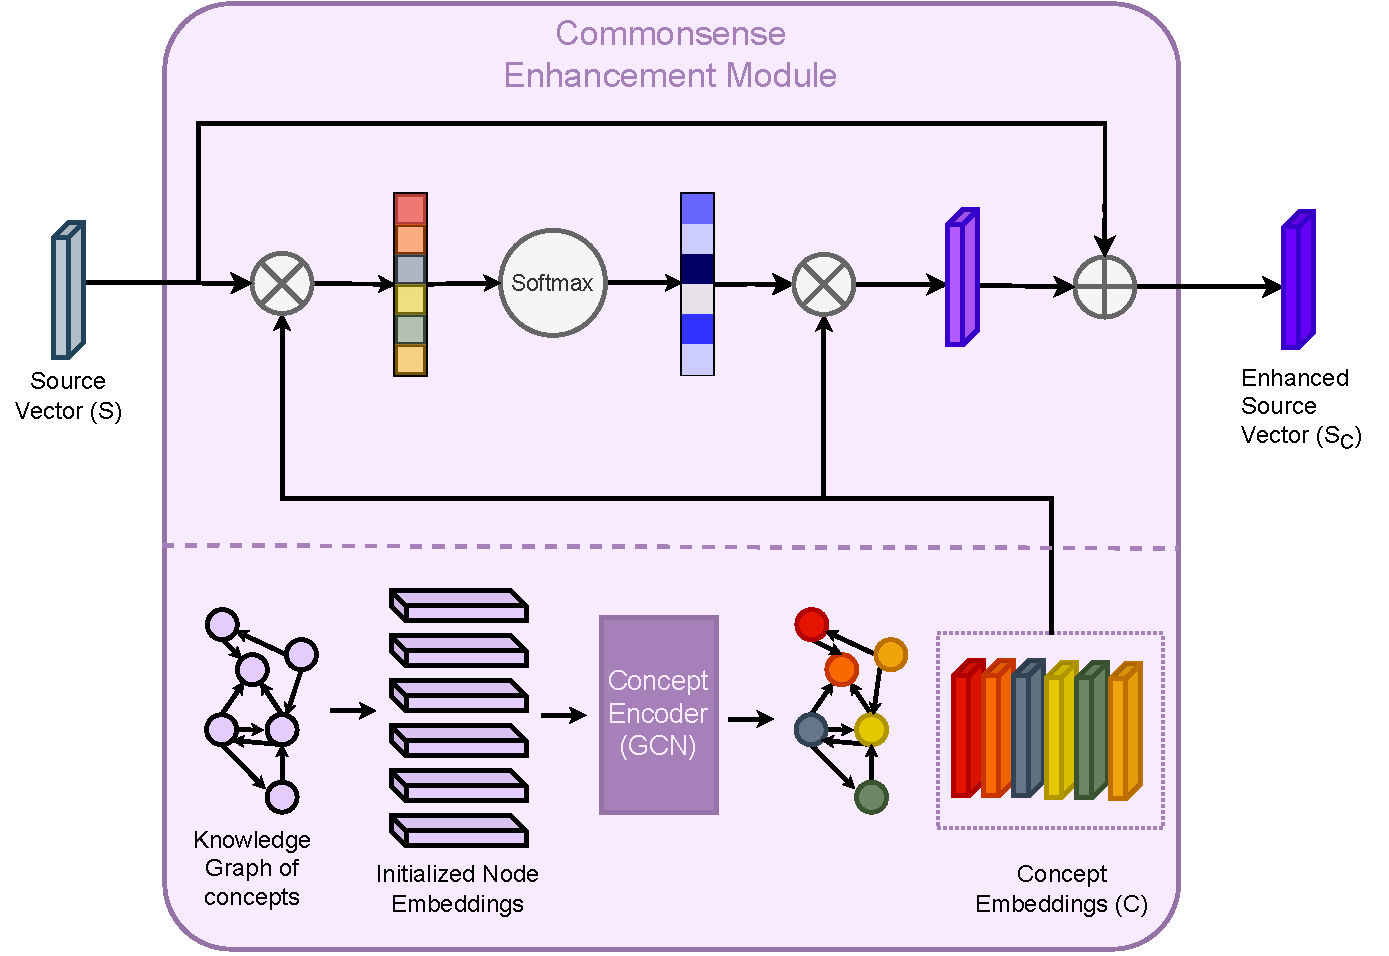
\includegraphics[width=0.8\linewidth]{figures/figure_files/Cem.pdf}
    \caption{\modelname Commonsense Enhancement Module (CEM). CEM comprises a concept encoder and an enhancement mechanism that uses the previously encoded concept vectors to update a given input vector (video/query vectors). The concept encoder employs a Graph Convolution Network for encoding the nodes (concepts) of \(G_C\). 
    }
  \label{fig:cem}
\end{figure}

CEM includes a set \(C\!=\!\left\{c_{1}, c_{2}, \dots, c_{n_{C}}\right\}\) of \(n_{C}\) concept vectors, where \(c_{i} \in \mathbb{R}^{d}\) and \(d\) is the concept feature dimension (same dimension as $\forall v_i \in V$ and $\forall q_i \in Q$). In general, given source feature vectors $S\!=\!\left\{ s_{1},s_{2},\ldots,s_{n}\right\}$ with individual feature vectors $s_{i \in [1,n]} \in \mathbb{R}^{d}$, the enhanced feature vectors $S_{C}$ are obtained using a commonsense enhancement mechanism $\phi_{C}$.
We implement this commonsense enhancement step $\phi_{C}$ as a cross-attention mechanism that enriches source input features, attending over $S$ guided by the commonsense concept vectors $C$, \ie, 
\begin{equation}
\label{eq:cenhance}
\scalemath{1}{
    }
    S_{C} = S + \phi_{C}(S) = S + \sigma \left( \frac{SW_{Q}(CW_{K})^{T}}{\sqrt{d}} \right) C W_{V},
\end{equation}
where $\sigma$ is a softmax activation, \(W_{Q}\), \(W_{K}\), \(W_{V}\) are trainable matrices and \(d\) is the common dimension of the vectors \(S\) and \(C\). In our setting, the source feature vectors $S$ are either video $V$ or pseudo-query $Q$ features. We build separate enhancement mechanisms for $V$ and $Q$, \ie, the projection matrices \(W_{Q}\), \(W_{K}\), \(W_{V}\) are not shared between $Q$ and $V$. We elaborate more on the rationale in the appendix.
The enriched video and pseudo-query features are denoted as \(V_{C}\!=\!\phi_{C_{\text{vid}}}(V)\) and \(Q_{C}\!=\!\phi_{C_{\text{pq}}}(Q)\), respectively.

\paragraph{Concept Encoder.}
The concept vectors \(C\) mentioned above are feature representations that internally form the nodes of the commonsense graph, \(G_C\). Accordingly, graph \(G_{C}\) is represented as a matrix, where \(G_{C(i,j)}\) represents the total number of directed relational edges between \(c_{i},c{j} \in C\) that start at \(c_i\) and end at \(c_j\). To encode the commonsense information, we employ Graph Convolutional Networks (GCN) \cite{hammond_wavelets_2011}. The concept encoder is composed of $L$ graph convolution layers, each of which performs a convolution step
\begin{equation}
\scalemath{1}{
    C^{\left(l+1\right)}=\sigma \left( AC^{\left(l\right) }W^{\left( l\right) }\right),
    }
\end{equation}
where $C^{\left(l\right)}$ are node (concept) features and $W^{\left( l\right)}$ trainable weight matrix of layer $l \in [1, L]$, $\sigma$ is a nonlinear activation function, and $A$ is the adjacency matrix obtained by normalizing graph $G_C$ with the degree matrix $D$. Since $G_C$ is a directed graph, normalization can be formulated as $A\!=\!D^{-1}G_{C}$.

\paragraph{Commonsense Information.}
We use ConceptNet \cite{speer_conceptnet_2017}, a popular knowledge graph that provides information spanning various types of relationships such as physical, spatial, behavioral, \etc To ensure that the ConceptNet information utilized is relevant to themes found in the video data, we consider the set of objects available in pseudo-queries and include the top-$k$ most frequently occurring objects to be the seed concept set \(C\). We extract the  ConceptNet subgraph that includes all edges incident between the concepts in \(C\). 
We filter the edge types based on a pre-determined relation set \(R\), which is compiled to involve relations that are relevant to the nature of the video localization task, \eg, spatial (\textit{AtLocation}, \etc) and temporal (\textit{HasSubevent}, \etc) relations are useful for video understanding, while \textit{RelatedTo} and \textit{Synonym} are fairly generic relations that add little information to the localization task. Table \ref{tab:relations} shows the relations included in \(G_C\).

\paragraph{Cross-Modal Interaction Module.} The commonsense enriched video and query features, \(V_{C}\) and \(Q_{C}\), are fused with a multi-modal cross-attention mechanism. We employ a two-step fusion process. First, Query-guided Video Attention (QVA) is applied to attend over video $V_C$, and Video-guided Query Attention (VQA) attends over query $Q_C$ guided by video $V_C$, resulting in updated features $V_C'$ and $Q_C'$, respectively. Both QVA and VQA utilize Attention Dynamic Filters~\cite{rodriguez_proposal-free_2020} that adaptively modify video features, dynamically adjusting them in response to the query, and vice versa. Next, the attended features are fused using a cross-attention mechanism over $V_C'$ guided by $Q_C'$, resulting in localized video features $V_{C_{\text{loc}}}$.

\paragraph{Temporal Regression Module.}
The final step involves a regression layer that approximates $\hat{V}_{\text{span}}$. We employ attention-guided temporal regression to estimate the span of the target video moment. To find important temporal segments relevant to the query, the fused features $V_{C_{\text{loc}}}$ are temporally attended based on the query features to obtain $V_{\text{ta}}$. Then, the span boundaries are localized using a regressor implemented as a Multi-Layer Perceptron (MLP).

\begin{align}
{o}_i = \sigma\left({W}_{1} V_{C_{\text{loc}_i}} + {b}_{{1}}\right) \\
V_{\text{ta}} = \sum_{i=1}^{T} o_i V_{C_{\text{loc}_{i}}} \\
[\hat{t}_s, \hat{t}_e] = {W}_2 {V}_{\text{ta}} + {b}_{2}.
\end{align}
Here, ${W}_{1}$ and ${b}_1$ are the weight matrix and bias vector of the temporal attention MLP, $\sigma$ represents the sigmoid activation function, $V_{C_{\text{loc}_i}}$ stands for the encoded localized video features, ${V}_{\text{ta}}$ represents the temporally attended video features, ${W}_2$ and ${b}_2$ denote the weight matrix and bias vector of the regression MLP, and $[\hat{t}_s, \hat{t}_e]$ correspond to the start and end timestamps of the predicted video span $\hat{V}_{\text{span}}$.

\begin{table}[t!]
\centering
\resizebox{\linewidth}{!}{
\begin{tabular}{ll}
\toprule
\textbf{Category} & \textbf{Relations}                                                                                         \\ \toprule
Spatial           & AtLocation, LocatedNear                                                                                    \\ \midrule
Temporal          & \begin{tabular}[c]{@{}l@{}}HasSubevent, HasFirstSubevent, HasLastSubevent, HasPrerequisite\end{tabular} \\ \midrule
Functional        & UsedFor                                                                                                    \\ \midrule
Causal            & Causes                                                                                                     \\ \midrule
Motivation        & MotivatedByGoal,  ObstructedBy                                                                             \\ \midrule
Other             & CreatedBy, MadeOf                                                                                          \\ \midrule
Physical          & \begin{tabular}[c]{@{}l@{}}HasA, HasProperty, Antonym, SimilarTo\end{tabular}                      
\\ \bottomrule
\end{tabular}
}

\caption{Relations in the Commonsense Enhancement Module (CEM) grouped by categories.}
\label{tab:relations}

\end{table}
\subsection{Training and Inference}
The training objective is 
$\mathcal{L}_{loc} = \mathcal{L}_{treg}+\lambda \mathcal{L}_{ta},$ where \(\lambda\) is a balancing hyperparameter, \(\mathcal{L}_{ta}\) is a temporal attention guided loss and \(\mathcal{L}_{treg}\) is the regression loss.  The temporal attention-guided loss is defined as
\begin{equation}
\label{tatt}
\mathcal{L}_{ta} = \frac{\sum^{T}_{i=1}g_{i}\log \left( a_{i}\right)}{\sum^{T}_{i=1}g_{i}},
\end{equation}
where \(a_{i}\) is the attention weight for video frame \(v_{i}\) and \(g_{i}\) is the attention mask for \(v_{i}\), that is assigned to \(1\) if \(v_{i}\) is inside the target video segment, and \(0\) otherwise. 
This objective encourages the model to produce higher attention weights for video segments that are relevant to the query. 
On the other hand, \(\mathcal{L}_{treg}\) dictates the video span boundary regression and is the sum of smooth $\ell_1$ distances between start and end timestamps of the ground truth and predicted spans, \ie,
\begin{equation}
\label{treg}
\mathcal{L}_{treg} = \text{smooth}{\ell_1}(t_{s}, \hat{t}_{s}) + \text{smooth}{\ell_1}(t_{e}, \hat{t}_{e}).
\end{equation}
Here, $t_{s}$ and ${t}_{e}$ represent the ground truth start and end timestamps and $\hat{t}_{s}$ and $\hat{t}_{e}$ the predicted start and end timestamps, respectively.
The integration of a smoothing mechanism enhances training stability and improves the model's ability to handle outliers. Finally, during inference, we employ an off-the-shelf part-of-speech tagger to extract nouns from the text input query and feed them as query input to the trained \modelname video localizer.

\section{Experiments}
\label{sec:experiment}

\begin{table}[t]
\centering
\small
\resizebox{0.99\linewidth}{!}{
\begin{tabular}{lcccc}
\multirow{2}{1.5cm}{\textbf{Methods}} & \multicolumn{2}{c}{\textbf{Far-OOD}} & \multicolumn{2}{c}{\textbf{Near-OOD}}\\
\cmidrule{2-5}
& \textbf{FPR95}  & \textbf{AUROC} & \textbf{FPR95}  & \textbf{AUROC}\\
& $\downarrow$ & $\uparrow$ & $\downarrow$ & $\uparrow$ \\
\toprule
\emph{Using model outputs}\\
MSP~\cite{hendrycks2016baseline} & 52.11 & 91.79 & 64.66 & 85.28 \\
ODIN~\cite{liang2018enhancing}  & 26.47 & 94.48 & 52.32 & 88.90\\
GODIN~\cite{hsu2020generalized}  & 17.42  & 95.84 & 60.69 & 82.37 \\
Energy score~\cite{liu2020energy}  & 28.40 & 94.22 & 50.64 & 88.66 \\
ReAct~\cite{sun2021react} & 33.12 & 94.32 & 53.51 & 88.96\\
GradNorm~\cite{huang2021importance} & 24.79 & 92.58 & 65.44 & 79.31\\
LogitNorm~\cite{wei2022mitigating}  & 19.61 & 95.51 & 55.08 & 88.03\\
DICE~\cite{sun2022dice}  & 20.83 & 95.24 & 58.60 & 87.11 \\
\midrule
\emph{Using feature representations}\\
Mahalanobis~\cite{lee2018simple} & 44.55 & 82.56 & 87.71 & 78.93 \\
KNN~\cite{sun2022knn}  & 18.50 & 96.36 & 58.34 & 87.90 \\
\midrule 
 \name (ours) & \textbf{14.99} & \textbf{97.15}  & \textbf{50.10} &  \textbf{89.80}\\
 & $\pm{0.87}$ & $\pm{0.27}$ & $\pm{1.09}$ & $\pm{0.65}$\\
\bottomrule
\end{tabular}}
\caption{\small Performance comparison on near-OOD and far-OOD detection task. Architecture used is DenseNet-101 and ID data is CIFAR-10. We report the mean and variance across 3 training runs.}
\label{tab:hard_ood}
\end{table}
\begin{table}[t]
\small
\centering
\resizebox{0.99\linewidth}{!}{
\begin{tabular}{lccc}
\textbf{Method} & \textbf{FPR95}  & \textbf{AUROC} & \textbf{ID Acc.}\\
& $\downarrow$ & $\uparrow$ & $\uparrow$ \\
\toprule
\emph{Methods using model outputs}\\
MSP~\cite{hendrycks2016baseline} & 77.59 & 76.47 &  75.14\\
ODIN~\cite{liang2018enhancing} & 56.39 & 86.02 & 75.14\\
GODIN~\cite{hsu2020generalized} & 44.08 &  89.05 & 74.37\\
Energy score~\cite{liu2020energy} & 57.07 &  84.83 &  75.14\\
ReAct~\cite{sun2021react} & 75.06 & 79.51 & 66.56\\
GradNorm~\cite{huang2021importance} & 63.05 & 79.80 & 75.14\\
LogitNorm~\cite{wei2022mitigating} & 61.10 & 84.72 & 75.42\\
DICE~\cite{sun2022dice} & 49.72 & 87.23 & 68.65 \\
\midrule 
\emph{Methods using feature representations}\\
Mahalanobis~\cite{lee2018simple} & 56.93 & 80.27 &  75.14\\
KNN~\cite{sun2022knn} & 47.21 & 85.27 & 75.14\\
\midrule 
 \name (ours) & \textbf{31.25} & \textbf{90.76} & \textbf{75.59}\\
& $\pm{1.25}$ & $\pm{0.36}$ & $\pm{0.08}$\\
\bottomrule
\end{tabular}}
\caption{\small Performance comparison on CIFAR-100 dataset. We use DenseNet-101 for all baselines. Best  results are in \textbf{bold}. We report the mean and variance across 3 different training runs.}
\label{tab:cifar-100}
\end{table}
In this section, we extensively evaluate the effectiveness of our proposed method. 
The goal of our experimental sections is to mainly answer the following questions: (1) Can \name alleviate the curse of dimensionality? (2) How does \name compare against the state-of-the-art OOD detection methods?  Due to space constraints, extensive experimental details are in Appendix C. Our code is open-sourced for the research community.


\subsection{Evaluation on Common Benchmarks}
\label{subsec:common_benchmark}

\noindent \textbf{Datasets.} In this section, we make use of commonly studied CIFAR-10 (10 classes) and CIFAR-100 (100 classes)~\cite{krizhevsky2009learning} datasets as ID. Both datasets consist of images of size $32 \times 32$. We use the standard split with $50,000$ images for training and $10,000$ images for testing. We evaluate the methods on common OOD datasets: \texttt{Textures}~\cite{cimpoi2014describing}, \texttt{SVHN}~\cite{svhn}, \texttt{LSUN-Crop}~\cite{yu2015lsun}, \texttt{LSUN-Resize}~\cite{yu2015lsun}, \texttt{iSUN}~\cite{xu2015turkergaze}, and \texttt{Places365}~\cite{zhou2017places}. Images in all these test datasets are of size $32 \times 32$. 


\paragraph{Evaluation metrics.} We compare the performance of various methods using the following metrics: 
(1) {FPR95} measures the false positive rate (FPR) of OOD samples when $95\%$ of ID samples are correctly classified;
(2) {AUROC} is the area under the Receiver Operating Characteristic curve; 
and (3) {ID Acc.} measures the ID classification accuracy.

\vspace{0.2cm}
\noindent \textbf{Comparison with competitive methods.} In Table~\ref{tab:cifar-100}, we provide a comprehensive comparison with competitive OOD detection baselines on  CIFAR-100. {We provide a detailed description of baseline approaches in Appendix C.3.} We observe that our proposed method \name significantly outperforms the latest rivals. For a fair comparison, we divide the baselines into two categories: methods using model outputs and methods using feature representations.
From Table~\ref{tab:cifar-100}, we highlight two salient observations: (1) Considering methods based on feature representations, \name outperforms KNN (non-parametric) and Mahalanobis (parametric) by \textbf{15.96\%} and \textbf{25.68\%} respectively in terms on FPR95. The results validate that learning feature subspace effectively alleviates the ``curse-of-dimensionality" problem that is troubling the existing KNN approach. (2) Further, \name also performs better than output-based methods such as ReAct~\cite{sun2021react}. Specifically, with CIFAR-100 as ID, \name provides a $\mathbf{43.81}\%$ improvement in FPR95 as compared to ReAct~\cite{sun2021react}. Notably, \name provides a \textbf{18.47\%} improvement compared to~\cite{sun2022dice}, a post-hoc sparsification method. While DICE can severely affect the ID test accuracy (68.65\%), \name exhibits stronger classification performance (75.59\%) by baking in the inductive bias of subspaces through training. An extensive discussion is provided in Section~\ref{sec:discussion}. 



\paragraph{Evaluation on near-OOD data.} In Table~\ref{tab:hard_ood}, we compare the performance in detecting near-OOD data, which refers to samples near the ID data. Near-OOD is particularly challenging to detect, and can often be misclassified as ID. We report the performance on CIFAR-10 (ID) vs. CIFAR-100 (OOD), which is the most commonly used dataset pair for this task. We observe that \name consistently outperforms existing algorithms for near-OOD detection tasks, further demonstrating its strengths. Compared to KNN, \name reduces the FPR95 by 8.24\%. For completeness, we also provide far-OOD evaluation results on CIFAR-10, where \name achieves an average FPR95 of 14.99\%. Full result on each test dataset for CIFAR-10 is available in Appendix D.4.



\begin{table}[t]
\small
\centering
\resizebox{0.95\linewidth}{!}{
\begin{tabular}{lccc}
\textbf{Method} & \textbf{Dataset (ID)} & \textbf{FPR95}  & \textbf{AUROC} \\
& & $\downarrow$ & $\uparrow$  \\
\toprule
Mahalanobis~\cite{lee2018simple} & CIFAR-10 & 44.55 & 82.56  \\

\name (w. Mahalanobis) & CIFAR-10 &  \textbf{34.68} &  \textbf{87.87} \\
\midrule
Mahalanobis~\cite{lee2018simple} & CIFAR-100 & 56.93 & 80.27  \\

\name (w. Mahalanobis) & CIFAR-100 &  \textbf{55.05} &  \textbf{80.77} \\
\bottomrule
\end{tabular}}
\caption{\small \name is also compatible with parametric approaches such as Mahalanobis distance~\cite{lee2018simple}. The model is DenseNet. All values are averaged over six OOD test datasets.}
\label{tab:compatibility}
\end{table}


\paragraph{Compatibility with other distance-based approaches.} 

Beyond KNN~\cite{sun2022knn}, the Mahalanobis distances~\cite{lee2018simple} is also one of the most popular distance-based approaches to detect OOD. 
However, all prior solutions measure the distance with a full feature space which can also suffer from the curse of dimensionality. 
In this section, we show that subspace learning can also benefit parametric approaches like Mahalanobis distance~\cite{lee2018simple}. In Table~\ref{tab:compatibility}, we compare the OOD detection performance of using Mahalanobis distance on the vanilla model and the model trained with \name. 
We see that coupling subspace learning (in training) with Mahalanobis distance (in testing) reduces FPR95 by {9.87\%} and {1.88\%} on CIFAR-10 and CIFAR-100 datasets respectively.

\begin{table}[t]
\small
\centering
\resizebox{0.55\linewidth}{!}{
\begin{tabular}{lcc}
\toprule
\multirow{2}{2cm}{\textbf{Training Method}} &  CIFAR-10 & CIFAR-100 \\ 
& \multicolumn{2}{c}{(Train time in hours)} \\
\midrule
Standard & $2.10$ & $2.25$\\ 
 \name & $1.75$ & $1.89$ \\
\bottomrule
\end{tabular}}
\caption{\small \textbf{Computational cost for training}. trained using ResNet-101. 
Model used is DenseNet-101. For the comparison, we used the software configuration as reported in Appendix C.2.}
\label{tab:train_time}
\end{table}
% 
\paragraph{Computational complexity.}  In Table~\ref{tab:train_time}, we compare the training time of \name with the standard training method using cross-entropy loss. We observe that training using \name incurs no additional computation overhead but rather is slightly more efficient compared to standard training procedures. This is because we perform gradient descent only on a subset of weights corresponding to the selected feature subspace. Thus, our method overall leads to faster updates and convergence. {In Appendix D.1, we further show that
\name remains competitive and outperforms the KNN counterpart on other common architecture.}

\section{Further Understanding of \name}
\label{sec:ablations}

Through comprehensive evaluations in Section~\ref{sec:experiment}, we have established the effectiveness of \name for OOD detection. 
\noindent In this section, we provide an in-depth analysis of several questions: (1) How does the subspace dimension impact the performance? (2) How does OOD detection performance change if we change the subspace selection strategy? 
(3) How does the $k$ in $k$-NN distance impact the OOD detection performance? We show comprehensive ablation studies to answer these questions. 
 For consistency, all ablations are based on CIFAR-100 as ID dataset and DenseNet~\cite{huang2018densely} architecture unless specified otherwise.
 

\begin{figure*}[t!]
\centering
\begin{minipage}{.49\textwidth}
  \centering
 \vspace{0.7cm}
  \includegraphics[width = 1\columnwidth]{images/Frame_6.pdf}
  \vspace{0cm}
    \caption{\small \textbf{Left}: Effect of varying the relevance ratio ($r$) on OOD detection performance when $k=20$. \textbf{Right}: Effect of varying the number of neighbors ($k$) when $r=0.25$. }

    \label{fig:ablations}
\end{minipage}
\hspace{0.1cm}
\begin{minipage}{.48\textwidth}
  \centering
\centering
    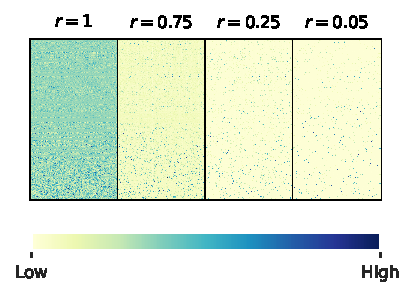
\includegraphics[width = 0.78\columnwidth]{images/subspace_new.pdf}
    \caption{
    \small Visualization of learned final-layer weight matrix for $r \in \{1, 0.75, 0.25, 0.05\}$. For each $r$, we visualize a $342$-dimensional weight vector corresponding to each class in CIFAR-100. }
    \label{fig:subspace}
\end{minipage}%


\end{figure*}
\paragraph{Ablation on subspace dimension.} In this ablation, we aim to empirically verify our theoretical analysis in Section~\ref{sec:theory}, and understand the effect of subspace dimension. 
We start by defining the \textbf{relevance ratio} $r = \frac{s}{m} \in (0,1]$, which captures the sparsity of feature space used in training \name. Recall that $m$ is the original dimension of features and $s$ is the dimension we kept in \name. 

In simple words, $r$ represents the ratio between the dimension of the subspace and the full feature dimension.
Specifically, we train and compare multiple models by varying $r = \{ 0.05, 0.15, 0.25, 0.35, 0.55, 0.75\}$. Figure~\ref{fig:ablations} (left) summarizes the effect of $r$ on OOD detection. We observe that: (1) Irrespective of the relevance ratio used, \name is consistently better than KNN~\cite{sun2022knn} when $r < 1$. This validates the efficacy of learning feature subspaces for OOD detection, without excessive hyperparameter tuning. (2) Setting a mild ratio (\emph{e.g.} $r=0.25$) provides the optimal OOD detection performance, which is consistent with one chosen using our validation strategy (see Appendix C.4). (3) In the extreme case, when $r$ is too small (\emph{e.g.} $r={0.05}$), we observe a deterioration in the OOD detection performance. Overall our empirical observations align well with our theoretical insight provided in Section~\ref{sec:theory}. 

\paragraph{Visualization of the learned weight matrix.}

To further verify our method, we visualize in Figure~\ref{fig:subspace} the 
learned final-layer weight matrix under different relevance ratios ($r = s/m$). For each $r$, we visualize the $342$ dimensional weight vector corresponding to each class in CIFAR-100, \emph{i.e.}, a $342 \times 100$ matrix. When $r=1$ (\emph{i.e.} without any subspace constraint), the model utilizes the full feature space. Further, the visualization confirms that decreasing the relevance ratio effectively reduces feature subspace dimensionality. 

\begin{table}[h]
\centering
\small
\resizebox{0.85\linewidth}{!}{
\begin{tabular}{lccc}
\textbf{Method} & \textbf{FPR95}  & \textbf{AUROC} \\
& $\downarrow $& $\uparrow$ \\
\toprule
Random subspace~\cite{ho1998nearest} & 42.21 & 84.97 \\
Subspace with least relevance & 63.96 & 80.82\\
\name (ours) & \textbf{31.25} & \textbf{90.76} \\
\bottomrule
\end{tabular}}
\caption{\small Ablation on subspace selection methods. Best performing results are marked in \textbf{bold}. Model is DenseNet. All values are averaged over multiple OOD test datasets.}
\label{tab:subspace-selection}
\end{table}


\paragraph{Ablation on subspace selection.} A core component of our algorithm involves selecting the  \emph{most relevant} dimension for a class prediction. In particular, the subspace is chosen based on the dimensions that contributed most to the model's output. In this ablation, we contrast our subspace selection mechanism with random subspace~\cite{ho1998nearest}, a classical alternative. The random subspace relies on a stochastic process that randomly selects $s$ components in the feature vector. Simply put, this approach randomly sets $s$ out of $m$ elements in each $R_c$ vector to be 1 and 0 elsewhere. We report ablation results  in Table~\ref{tab:subspace-selection}. For a fair comparison, we use relevance ratio $r = 0.25$ and the number of neighbors $k = 20$ for all methods.  Empirical results highlight that randomly chosen subsets of dimensions are sub-optimal for the OOD detection task. Lastly, we also contrast with selecting the \emph{least relevant} feature dimensions. We replace Equation~\ref{eq:relevance} with: 
\begin{align}
     f_c(\*x; \theta, R_c(\*x)) & =  \min_{R_c(\*x)\in \{0,1\}^m, \|R_c(\*x)\|_1 = s} \langle \*w_c, h(\*x) \odot R_c(\*x) \rangle,
     \label{eq:least_relevance}
\end{align}
which essentially changes from \textsc{max} to \textsc{min}.  As expected, using the least relevant feature dimension results in significantly worse OOD detection performance.


\paragraph{Ablation on number of nearest neighbors $k$.} 
In Figure~\ref{fig:ablations} (right), we visualize the effect of varying the number of nearest-neighbors ($k$) on OOD detection performance. Here the model is trained with $r=0.25$ on CIFAR-100. Specifically, we vary $k \in \{5,10,20,50,100,200,500,1000\}$. We observe that the  OOD detection performance is relatively stable under a mild $k$. In Appendix D.2, we further visualize the interaction between the two hyper-parameters $r$ and $k$ through OOD detection performance. 

\vspace{0.1cm}
\noindent\textbf{\name improves calibration performance.} {
In addition to superior OOD detection performance, we aim to further  investigate the calibration performance of ID data itself. As a quick recap,  the calibration performance measures the alignment between the model's confidence and its actual predictive accuracy. We hypothesize that learning the feature subspace helps alleviate the problem of over-confident predictions on ID data, thereby improving model calibration. We verify in  Appendix D.3 that training with \name indeed significantly improves the model calibration. }

\vspace{0.1cm}
\noindent\textbf{\name scales to large datasets.} 
In this section, we evaluate \name on a more realistic high-resolution dataset ImageNet ~\cite{deng2009imagenet}. Compared to CIFAR-100, inputs scale up in size in ImageNet-100 (we follow standard data augmentation pipelines and resize the input to 224 by 224). For OOD test datasets, we use the same ones in~\cite{huang2021mos}, including subsets of \texttt{Places365}, \texttt{Textures}, \texttt{iNaturalist} and \texttt{SUN}. 
We train the ResNet-101 model for 100 epochs using a batch size of 256, starting from randomly initialized weights. We use SGD with a momentum of $0.9$, and a weight decay of 1e-4. We set the initial learning rate as $0.1$ and use a cosine-decay schedule. We set $r = 0.35$ and $k = 200$ based on our validation strategy described in Appendix C.4. We contrast two models trained with and without subspace learning. The results in terms of FPR95 and AUROC are shown in Figure~\ref{fig:imagenet}. The results suggest that \name remains effective on all the OOD test sets and consistently outperforms KNN. This further verifies the benefits of explicitly promoting feature subspace to combat curse-of-dimensionality. 

\begin{figure}[t]
    \centering
    \includegraphics[width = \linewidth]{images/imagenet_plot.pdf}
    \caption{\small OOD detection performance comparison on ImageNet dataset (ID). \name consistently outperforms KNN across all OOD test datasets on the same architecture.  }
   
    \label{fig:imagenet}
\end{figure}



\section{Discussion}\label{sec:discussion}
%<insert>
%In this section we discuss the helpfulness of a theoretical ``audit standard'' to study content curators and note how our framework might contribute to such a standard. We also note the various audit methods used in this study and clarify the strengths of the different methods. In regards to the audit results, we discuss possible motivations for the mechanism design 
In this section we first discuss the specific results found in our audit of Apple News and how our results paint a distinction between algorithmic logic and human editorial logic. We then consider the broader implications of our study in terms of the various audit methods used, clarifying their different strengths. And finally, we suggest that the audit framework we develop may contribute to informing a conceptual ``audit standard'' which helps make the questions and methods more consistent when approaching similar audits of other news curators. 


\subsection{Mechanisms behind Apple News}
The absence of localization and personalization in the sections we audited highlights a possible tension between equitable economic distribution and vulnerability to echo-chambers. By showing the same Top Stories and Trending Stories to every user, Apple has taken a measure that minimizes individual filter bubble effects. However, this design choice may also translate to a highly-skewed distribution of economic winnings for publishers, since the few sources that frequent the top slots reap disproportionate traffic and potential advertising revenue from the 85 million users. 

Certainly, a balance could mitigate filter bubble effects while creating more equitable monetization. For example, Google News provides all users with an algorithmically-selected five-story briefing, but the same two top stories are shown to all users \citep{Wang2018}. Apple might explore a similar hybrid approach, using their editorial team to choose a mix of regionally and nationally relevant news. It should also be noted that Apple News includes a ``For You" section based on ``topics \& channels you read," which may help balance these tensions. 


\subsection{Algorithmic vs. Editorial Logic}
Our results illustrate what \citet{Gillespie2014} refers to as a possible competition between ``editorial logic'' and ``algorithmic logic.'' While the algorithmic logic behind Trending Stories is intended to ``automate some proxy of human judgment or unearth patterns across collected social traces,'' the editorial logic behind Top Stories ``depends on the subjective choices of experts, themselves made and authorized through institutional processes of training and certification'' \citep{Gillespie2014}. These logics manifest in our audit results for both mechanism and  content: Trending Stories and Top Stories exhibit distinct update schedules, sources, and topics that reflect their respective logics.

According to interviews with Apple's staff by \citet{Nicas2018}, the editorial logic behind the Top Stories pushes new content ``depending on the news,'' and also ``prioritizes accuracy over speed.'' In contrast, the Trending Stories section continually churns out new content (over 50 stories per day on average, more than twice as many as the Top Stories section). The algorithmic logic continually updates `what's trending,' and does so at all hours of the day (see Figure \ref{fig-trending-stories-appearance-times}), whereas the editorial logic espoused by Apple's staff strives for ``subtly following the news cycle and what's important'' \citep{Nicas2018}.

The contrast in logics extends to source concentration and source diversity. The editorially-selected Top Stories section exhibited more diverse and more equitable source distribution than the algorithmically-selected Trending Stories, as detailed in Table \ref{summary-table} and visualized in Figures \ref{fig-trending_stories_distribution} and \ref{fig-top_stories_distribution}. During the two-month data collection, human editors chose from a slightly wider array of sources than the algorithm behind Trending Stories, and also distributed selections more equitably across those sources, although there was a core set of 40 sources that were selected by \textit{both} algorithm and editor. Apple's editors also appeared to seek out regional news sources when the topic called for it. For example, during our data collection, the team chose stories from The San Diego Union-Tribune, The Miami Herald, The Chicago Tribune, TwinCities.com, and The Baltimore Sun. While the Trending Stories algorithm surfaced some content from smaller sources (e.g., esimoney.com, a single-author website dedicated to money management), no sources were regionally-specific.

Finally, perhaps the most intuitive distinction between the editorial logic and the algorithmic logic exhibited in Apple News is differences in content. Trending Stories uniquely included ``soft news'' \citep{Reinemann2012} pieces about celebrities and entertainment (ex. Kate Middleton, Justin Bieber), while the Top Stories uniquely included ``hard news'' topics including international stories and news about political policy (ex. Brexit, Affordable Care Act). Our data corroborates initial reports that headlines in Trending Stories ``tend to focus on Mr. Trump or celebrities'' \citep{Nicas2018}.


\subsection{Broader Implications}

\subsubsection{Audit Methods}
To study Apple News we used scraping, sock-puppet, and crowdsourced auditing. While these techniques have been employed in previous audit studies, we next reflect on our experience of how we found each technique helpful for addressing different aspects of our audit framework, in hopes this can inform future audit studies. 

First, audit studies should consider crowdsourcing whenever real-world observation is important, or when seeking higher parallel throughput in the data collection process. By using the crowd, we were able to assess the degree of personalization Apple News performs in practice, rather than fully relying on simulated sock-puppet data. Also, since resource constraints limited us to run at most two simulators at a time, crowdsourcing allowed us to significantly increase the throughput of our data collection, as many crowd workers could take screenshots in parallel.

Sock-puppet auditing -- using computer programs to impersonate users \citep{Sandvig2014} -- is most helpful for isolating variables that might affect a given system. Sock puppets provide clear and precise information about the input to an algorithm in cases where the crowd falls short. For example, precise temporal synchronization was still challenging with crowdworkers, as 6.7\% of screenshots from the crowd showed times that did not match the requested time in minutes, and even screenshots at the correct hour and minute may have been unsynchronized if seconds were taken into account. On the other hand, when using sock puppets, we could perform time-locked data collection on multiple devices with same-second precision.
%fine-grained location reporting is invasive: in a pilot study we attempted collecting ZIP codes, which some crowd workers either forged or simply declined to report. However, when using sock puppets, we could precisely situate the device at a given latitude and longitude while guaranteeing the absence of other factors such as user-level blocked sources. 

Lastly, we found the scraping audit most helpful for extended data collection, and we suggest scraping whenever researchers seek continuous data or to monitor over time. While we initially deployed a crowdsourced method for the extended data collection \citep{Bandy}, we found that we could not rely on the crowd for consistent data over time. Namely, in the United States, it was difficult to collect screenshots between the hours of 1am and 5am. However, after observing no evidence of personalization or localization in our initial experiments, we needed data from just one user account. We could therefore scrape content from a single simulated device to run the extended data collection.

It should be noted that we categorize our Appium-based data collection as a scraping audit since it centers around ``repeated queries to a platform and observing the results'' \citep{Sandvig2014}, however, we used a simulated iPhone to impersonate a user, making it somewhat of a hybrid with sock-puppet auditing. The Apple News platform lacks a public or private endpoint from which to scrape stories, so our experiment required additional layers of operation -- every data point we collected required simulating a user opening the application, refreshing for new content, locating buttons, and pressing buttons, thus requiring more time to collect data compared to a traditional scrape.

\subsubsection{Audit Framework}
To guide this work, we developed a conceptual framework that articulates three common aspects of a curation system that an audit might address: mechanism, content, and consumption. We showed how each of these aspects can have consequences for individual users, publishing companies, and even political discourse. As news curation systems change, consequential aspects may also change and prompt an expanded or revised framework.

Still, future research might leverage our proposed framework for auditing other content curators, revising and elaborating it to suit the nuances of specific systems. We believe this framework helps advance towards a conceptual ``audit standard'' for curation systems, which might allow the research community to compare and contrast different curation platforms, as well as characterize the evolution of a single platform over time.




\textbf{Language conditioned manipulation.} 
Significant work has been performed in  learning concepts and tasks for robots in interactive settings~\cite{gopalan2018sequence,gopalan2020simultaneously,tellex2020robots} even with the use of dialog~\cite{chai2018language,matuszek2012joint}.
Our work differs from previous works as it learns visual concepts for manipulation one-shot, and improves generalization by updating other known concepts.
Moreover, our approach can learn a concept hierarchy starting from zero known concepts, displaying the adaptability of our model under a continual learning setup.
%Our work differs from previous works as it is attempting to learn visual concepts for manipulation one-shot, while updating other known concepts to improve generalization.
%Moreover, our approach is completely differentiable and can start with zero known concepts, which is important for a continual learning setup. 
Previous work has focused on language conditioned manipulation~\citep{shridhar2021cliport, liu2021structformer, brohan2023rt1, brohan2023rt2}. \citealt{shridhar2021cliport} computes a pick and place location conditioned on linguistic and visual inputs. 
\citealt{liu2021structformer} focuses on semantic arrangement on unseen objects. 
Other works train on large scale linguistic and visual data and can perform real-life robotic task based on language instructions~\citep{ahn2022i, brohan2023rt1, brohan2023rt2}. Our work focuses on interactive teaching of tasks and concepts instead of focusing on the emergent behaviors from large models. 
% \citealt{ahn2022i} uses a pre-trained to propose plans to complete task and executes the feasible grounded plan. 
% None of these approaches discussed above focus on one shot teaching of concepts and task types to solve novel tasks in a zero-shot setting.
\citealt{daruna2019robocse} learns a representation of a knowledge graph by predicting directed relations between objects allowing a robot to predict object locations. 
To the best of the author's knowledge, our work  is the first that learns concepts and tasks one-shot to generalize to novel task scenarios on a robot, making our contributions significant compared to other related works.   


\noindent\textbf{Visual reasoning and visual concept learning.} Our work is related to visual concept learning \citep{mei2022falcon, mao2018the, yi2019neuralsymbolic, han2020visual, li2020competenceaware} and visual reasoning \citep{Mascharka_2018, DBLP:journals/corr/abs-1807-08556, DBLP:journals/corr/JohnsonHMHLZG17, DBLP:journals/corr/abs-1803-03067}. To perform the visual reasoning task, traditional methods \citep{Mascharka_2018, DBLP:journals/corr/abs-1807-08556, DBLP:journals/corr/JohnsonHMHLZG17, DBLP:journals/corr/abs-1803-03067} decompose the visual reasoning task into visual feature extraction and reasoning by parsing the queries into executable neuro-symbolic programs.  On top of that, many concept learning frameworks \citep{mei2022falcon, mao2018the, yi2019neuralsymbolic, han2020visual, li2020competenceaware} learn the representation of concepts by aligning concepts onto objects in the visual scene. 
% \ngnote{\citealt{yi2019neuralsymbolic} parses the visual scene into a structural scene representation, which makes the results of the neural network more interpretable.  \citealt{mao2018the} presents a concept learner that jointly learns a visual feature extractor, visual concept representation, and semantic parsing. \citealt{han2020visual} shows that introducing the relationships between concepts and higher-level concepts is helpful in learning the concept’s representation. \citealt{mei2022falcon} even shows that it is possible to train a module that learns a new concept with a very limited number of examples and its conceptual relationship to known concepts.} 
As far as we know, \citealt{mei2022falcon}'s FALCON is the most similar work to our work in this line of research. However, when introducing a new concept, our work continually updates the representation of all related concepts, whereas \citealt{mei2022falcon} does not, which makes it ill-suited for continual learning settings. Our work is also related to the area of few-shot learning~\citep{snell2017prototypical, tian2020rethinking, vinyals2017matching}, which learns to recognize new objects or classes from only a few examples but does not represent a concept hierarchy which is useful in robotics settings.



% \textbf{Few-shot learning.} Our work is also related to the area of few-shot learning, which learns to recognize new objects or classes from only a few examples. \citealt{vinyals2017matching} and \citealt{snell2017prototypical} use the visual features of a small number of annotated images as representation for the new class. 
% While the existing frameworks use Euclidean distance or cosine similarity to compute similarity between classes, \citealt{sung2018learning} trains a learnable module to predict the similarity between examples. Provided the relationship between the new class and known class, \citealt{wang2018zeroshot} and Kampffmeyer et al. \cite{kampffmeyer2019rethinking} learn the representation of a new class with no visual example. \citealt{tian2020rethinking} trains a transferable embedding model that can generalize to new classes. 

% \textbf{Continual learning and knowledge graphs.} Another area of work related to ours is continual learning and knowledge graphs. \citealt{daruna2019robocse} learn a representation of a knowledge graph by predicting whether a directed edge between two vertices is within the graph or not. On top of the existing framework, \citealt{daruna2021continual} shows that it is possible to continually update the knowledge graph whenever a new edge or a new vertex appears while avoiding catastrophic forgetting. 

\noindent\textbf{Scene graph.} Scene graphs are  structural representations of all objects and their relationships within an image. The scene graph representation~\cite{Chang_2023} of images is widely used in the visual domains for various tasks, such as image retrieval\cite{DBLP:journals/corr/JohnsonHMHLZG17}, image generation\citep{johnson2018image}, and question answering\citep{teney2017graphstructured}.
This form of representation has also been used in the robotics domains 
% combines geometric scene graph and symbolic scene graph as a representation of the scene 
for long-horizon manipulation~\citep{zhu2021hierarchical}.

\section{Conclusion}
In this paper, we introduced a new ad-hoc retrieval approach GRMM which explicitly incorporates document-level word relationships into the matching function. The flexible graph structure allows the model to find more comprehensive matching patterns and less noises. GRMM exceedingly advances the performance over various baselines, where it empirically witnesses an increment by a large margin on longer documents. Further studies exhibited the rationality and effectiveness of GRMM. There are also possible extensions, such as training with large click logs \cite{jiang2016learning} and query descriptions. Another interesting future work is to extend the current graph with lexical or knowledge graphs which might contain more useful information. 

\section*{Acknowledgement}
Research is supported by the AFOSR Young Investigator Program under award number FA9550-23-1-0184, National Science Foundation (NSF) Award No. IIS-2237037 \& IIS-2331669, Office of Naval Research under grant number N00014-23-1-2643, and faculty research awards/gifts from Google and Meta.  Any opinions, findings, conclusions, or recommendations
 expressed in this material are those of the authors and do not necessarily reflect the views, policies, or endorsements either expressed or implied, of the sponsors.

Odit deleniti ipsam possimus est quas inventore recusandae sint ad, labore suscipit est debitis facilis earum ipsam, rem ratione itaque iure ipsa est animi illo eaque quod, a aliquam sunt aut laboriosam necessitatibus qui culpa?Debitis asperiores suscipit ducimus, deserunt voluptatum temporibus tempora magni facere praesentium id totam aspernatur illo sapiente, illo hic similique fugiat temporibus quisquam dicta iste perspiciatis nobis alias, ducimus qui provident est temporibus porro a voluptate at dicta, facilis laboriosam laborum quibusdam quasi provident neque dolore cupiditate voluptatum a.Perferendis quo doloremque amet itaque veniam saepe incidunt atque illo beatae, esse vero aperiam velit fuga ad?Amet consequuntur voluptas vero commodi, excepturi hic reiciendis earum sunt.Odit dolore nisi porro quae placeat voluptas labore excepturi autem reprehenderit sed, laudantium ullam mollitia eligendi adipisci obcaecati sit consequatur blanditiis, tempora totam doloremque commodi earum quidem reprehenderit distinctio, ad sint deserunt, expedita fuga asperiores optio quaerat?Recusandae ipsum culpa cupiditate autem ab totam officia sit consequatur similique sint, maiores corporis nihil.Saepe libero beatae voluptatibus ab a magni officia rem, aliquid doloremque odio, doloribus culpa atque cumque quo, non voluptas minima nesciunt autem laborum similique adipisci eveniet porro deleniti quia, neque eligendi architecto.Delectus magni corrupti sit non, temporibus quidem accusamus nesciunt itaque blanditiis impedit molestiae alias maiores dolore commodi, quam sapiente aliquid nisi obcaecati sint.Architecto quis in deleniti molestias ad debitis eveniet natus, voluptas saepe aliquid unde doloremque, ut fuga hic esse debitis, accusantium excepturi omnis nisi illo quasi.Magni deleniti distinctio nam porro mollitia quae unde quis commodi iusto quia, minima ipsam doloremque, perferendis nesciunt delectus sequi quis non eligendi, expedita earum itaque ratione aut tenetur ad animi, suscipit eius unde illum accusamus ratione laboriosam ipsa cum?Aliquam fugit cumque rerum est, minus quo quod dignissimos nisi velit provident autem iste.Delectus ullam officia expedita reiciendis ipsam modi maiores quidem natus, illo explicabo quibusdam nesciunt voluptatum id earum at, distinctio deleniti corrupti architecto dolores quis amet itaque soluta, culpa omnis ipsa recusandae debitis.Hic aperiam quasi ipsa recusandae voluptatem ab distinctio tempora ad, consequatur odio ut voluptas hic, enim libero sint dolores culpa?Omnis doloremque animi provident unde aut maiores tempore recusandae, enim quo reprehenderit illo nihil eaque voluptate accusantium eligendi, veniam iusto dolore officia aliquid laborum dolorum impedit consectetur?Debitis officia labore, a consequatur saepe voluptatibus temporibus qui earum numquam officiis eaque assumenda impedit.Repudiandae similique necessitatibus adipisci, in blanditiis obcaecati ex veniam explicabo?Officia blanditiis quas culpa sint, minima iure iste, ab cum exercitationem.Sed beatae sint consectetur perspiciatis dolor temporibus, quod consequatur facere, nostrum culpa deserunt facilis autem voluptates nesciunt quidem dignissimos aperiam rerum voluptatum, quidem aut eaque a culpa obcaecati saepe quam laborum veritatis accusantium exercitationem?Officia debitis quo, ipsum quod illo repellat laborum id illum pariatur, omnis in tenetur maiores at.\clearpage
\bibliography{egbib}
\clearpage

\appendix
\section{Societal Impact}
\label{sec:impact}
In this paper, we show that in high-dimensional spaces, the efficacy of distance-based out-of-distribution (OOD) detection methods can be limited by curse-of-dimensionality. To combat this problem, we propose a novel framework of subspace learning for OOD detection. OOD detection is a critically important component for a vast range of systems which include
business applications (e.g., content understanding), transportation (e.g., autonomous vehicles), and health care (e.g., unseen disease identification). Our study has positive societal impacts. We hope that it will further enhance the understanding regarding the crucial issue of how curse-of-dimensionality affects distance-based OOD detection methods. Our study does not involve any human subjects or violation of legal compliance. We do not anticipate the potentially harmful consequences of our work. Through our study and releasing our code, we hope to raise stronger research and societal attention to the problem of OOD detection.

\section{Proof of Main Theorem}
\label{app:proof}

\begin{theorem} (Recap of Th.~\ref{th:main}) We let $\mathbb{E}[p_{in}(\*z)|{\*z \in \mathcal{Z}_{in}}] - \mathbb{E}[p_{in}(\*z)|{\*z \in \mathcal{Z}_{out}}] = \Delta(m)$ as a function of the feature's dimensionality $m$. We have the following bound:
    \begin{align}
            \hat{\Delta}(m) & \geq \Delta(m) - O((\frac{k}{N})^{\frac{1}{m}} + k^{-\frac{1}{2}})
    \end{align}
\label{th:sup_main}
\end{theorem}

\begin{proof}

\begin{align*}
     &\mathbb{E}[p_{in}(\*z)|{\*z \in \mathcal{Z}_{in}} ]  - 
    \mathbb{E}[p_{in}(\*z)|{\*z \in \mathcal{Z}_{out}}]
    \\ 
    &~~=  \mathbb{E}[p_{in}(\*z) - \hat{p}_{in}(\*z)|{\*z \in \mathcal{Z}_{in}}] + 
    \mathbb{E}[\hat{p}_{in}(\*z)|{\*z \in \mathcal{Z}_{in}}] \\
    &~- \mathbb{E}[\hat{p}_{in}(\*z)|{\*z \in \mathcal{Z}_{out}}] +
    \mathbb{E}[\hat{p}_{in}(\*z) - p_{in}(\*z)|{\*z \in \mathcal{Z}_{out}}] 
    \\ &~~\leq  \mathbb{E}[|p_{in}(\*z) - \hat{p}_{in}(\*z)| | {\*z \in \mathcal{Z}_{in}}] + 
    \mathbb{E}[\hat{p}_{in}(\*z)|{\*z \in \mathcal{Z}_{in}}]\\
    &~- \mathbb{E}[\hat{p}_{in}(\*z)|{\*z \in \mathcal{Z}_{out}}] +
    \mathbb{E}[|\hat{p}_{in}(\*z) - p_{in}(\*z)| | {\*z \in \mathcal{Z}_{out}}] 
    \\
    &~~= \frac{\int_{\mathcal{Z}_{in}} |p_{in}(\*z) - \hat{p}_{in}(\*z)| p_{in}(\*z) d\*z }{\int_{\mathcal{Z}_{in}}  p_{in}(\*z) d\*z } \\
    &~+ \frac{\int_{\mathcal{Z}_{out}} |p_{in}(\*z) - \hat{p}_{in}(\*z)| p_{in}(\*z) d\*z }{\int_{\mathcal{Z}_{out}}  p_{in}(\*z) d\*z }  \\
    &~+  \mathbb{E}[\hat{p}_{in}(\*z)|{\*z \in \mathcal{Z}_{in}}] - \mathbb{E}[\hat{p}_{in}(\*z)|{\*z \in \mathcal{Z}_{out}}]\\
    \\ &\leq \frac{\int_{\mathcal{Z}_{in}} |p_{in}(\*z) - \hat{p}_{in}(\*z)| p_{in}(\*z) d\*z  + \int_{\mathcal{Z}_{out}} |p_{in}(\*z) - \hat{p}_{in}(\*z)| p_{in}(\*z) d\*z }{\min(\int_{\mathcal{Z}_{in}}  p_{in}(\*z) d\*z, \int_{\mathcal{Z}_{out}}  p_{in}(\*z) d\*z) }\\
    &~+ \mathbb{E}[\hat{p}_{in}(\*z)|{\*z \in \mathcal{Z}_{in}}] - \mathbb{E}[\hat{p}_{in}(\*z)|{\*z \in \mathcal{Z}_{out}}] \\
    \\ &~~= \frac{\int_{\mathcal{Z}} |p_{in}(\*z) - \hat{p}_{in}(\*z)| p_{in}(\*z) d\*z  }{\min(\int_{\mathcal{Z}_{in}}  p_{in}(\*z) d\*z, \int_{\mathcal{Z}_{out}}  p_{in}(\*z) d\*z) } \\
    &~+ \mathbb{E}[\hat{p}_{in}(\*z)|{\*z \in \mathcal{Z}_{in}}] - \mathbb{E}[\hat{p}_{in}(\*z)|{\*z \in \mathcal{Z}_{out}}]
    \\ &~~= \frac{\mathbb{E}[|p_{in}(\*z) - \hat{p}_{in}(\*z)|] }{\min(\int_{\mathcal{Z}_{in}}  p_{in}(\*z) d\*z, \int_{\mathcal{Z}_{out}}  p_{in}(\*z) d\*z) } \\
    &~+ \mathbb{E}[\hat{p}_{in}(\*z)|{\*z \in \mathcal{Z}_{in}}] - \mathbb{E}[\hat{p}_{in}(\*z)|{\*z \in \mathcal{Z}_{out}}].
\end{align*}


\begin{lemma}
According to Theorem 1 in ~\cite{zhao2022analysis}, the estimation error of $k$-NN distances can be bounded by:
$$
\mathbb{E}[|p_{in}(\*z) - \hat{p}_{in}(\*z)|]  \leq \mathcal{O}(\left(\frac{k}{N}\right)^{\frac{1}{m}} + k^{-\frac{1}{2}})
$$
\label{lemma:est_err}
\end{lemma}
By Lemma~\ref{lemma:est_err}, we have the final results: 
\begin{align*}
     \mathbb{E}[\hat{p}_{in}(\*z)|{\*z \in \mathcal{Z}_{in}}] - & \mathbb{E}[\hat{p}_{in}(\*z)|{\*z \in \mathcal{Z}_{out}}] \geq \mathbb{E}[p_{in}(\*z)|{\*z \in \mathcal{Z}_{in}} ] \\
     &- \mathbb{E}[p_{in}(\*z)|{\*z \in \mathcal{Z}_{out}}] - O((\frac{k}{N})^{\frac{1}{m}} + k^{-\frac{1}{2}})
\end{align*}

\end{proof}



\section{Supplementary Experiment Details}
\label{app:experimental_details}
 \subsection{Training details}
\label{app:train_details}
For main experimentation, we train DenseNet-101~\cite{huang2018densely} for 100 epochs using SGD with a momentum of 0.9, a weight decay of 0.0005, and a batch size of 64. We set the
initial learning rate as 0.1 and reduce it by a factor of 10 at 50, 75, and 90 epochs. For ResNet-50~\cite{he2016deep}, we use SGD with a momentum of 0.9, weight decay of 0.0001, batch size of 128, and train the model for 100 epochs. The learning rate is adjusted using the same schedule as used for training the DenseNet model.
The relevance ratio $r \in \{0.05, 0.15, 0.25, 0.35, 0.55, 0.75\}$ and number of neighbors $k \in \{5,10,20,50,100,200,500,1000\}$ are cross-validated as described in Appendix~\ref{app:validation}. For all experiments on CIFAR-10/100 benchmark using DenseNet~\cite{huang2018densely}, we use $r=0.25$ and $k=20$ based on our validation strategy. For experimentation using ResNet-50~\cite{he2016deep}, we set $r=0.05$ and $k=20$. We report ablation results for the effect of $r$ and $k$ in Section~\ref{sec:ablations}.

\subsection{Software and Hardware}
\label{app:hardware}
We run all experiments with Python 3.7.4 and PyTorch 1.9.0. For all experimentation, we use Nvidia RTX 2080-Ti and A6000 GPUs.


\subsection{Description of OOD baselines}
\label{app:ood_description}
In this section, we include a brief description of all the OOD baseline methods.
\subsubsection{Methods using model outputs}


\paragraph{Maximum Softmax Probability (MSP)~\cite{hendrycks2016baseline}} uses the maximum softmax probability (or the confidence score) to detect OOD examples.

\paragraph{ODIN~\cite{liang2018enhancing}} ODIN utilizes the confidence score after temperature scaling and input perturbations for OOD detection. We set temperature parameter $T=1000$ for all experiments on the CIFAR-10/100 benchmark. Perturbation Magnitude $\eta$ is chosen by validating on 1000 images randomly sampled from the ID test set. We set the perturbation magnitude $\eta = 0.0016$ for CIFAR-10 and $\eta = 0.0012$ for CIFAR-100.

\paragraph{Energy~\cite{liu2020energy}} Liu~\etal~proposed using energy score for OOD detection. The energy function maps the logits to a scalar output, which is relatively
lower for ID data. This score is hyperparameter free and does not require any tuning.


\paragraph{Generalized-ODIN \cite{hsu2020generalized}} Hsu \etal~propose a decomposed confidence model for the purpose of OOD detection, where the logits of a classifier are defined using a dividend/divisor structure. The authors propose three variants of OOD detectors, namely, DeConf-I, DeConf-E, and DeConf-C --- which uses Inner-Product, Negative Euclidean Distance, and Cosine Similarity respectively. In this study, we use the DeConf-C variant, since it is shown to be the most robust of all the variants. Finally, input samples are perturbed to improve OOD performance. Similar to ODIN~\cite{liang2018enhancing}, the perturbation magnitude $\epsilon$ is chosen by validating on 1000 images randomly sampled from the ID test set. We set perturbation magnitude $\epsilon = 0.02$ for both CIFAR-10/100 benchmarks.

\paragraph{ReAct~\cite{sun2021react}} ReAct is a post-hoc OOD detection approach based on activation truncation. The paper states that the optimal OOD performance is obtained with the ReAct+Energy setting. Hence, in this study, we use the energy score for OOD detection using ReAct. Following the original paper, we calculate the clipping threshold based on the $90$-th percentile of activations estimated on the ID data.

\paragraph{GradNorm~\cite{huang2021importance}} GradNorm employs the magnitude of gradient vectors for detecting OOD samples. The gradient is derived from the KL-divergence between the softmax output and uniform probability distribution. For GradNorm, following the original implementation, we set the temperature $T = 1$.

\paragraph{LogitNorm~\cite{wei2022mitigating}} LogitNorm proposes a simple fix to the common cross-entropy loss by enforcing a constant vector norm on the logits during training. A temperature parameter $\tau$ is used to modulate the magnitude of the logits. In this study, we set $\tau = 0.04$ for both CIFAR-10/100 datasets.

\paragraph{DICE~\cite{sun2022dice}} DICE ranks weights based on a measure of contribution, and selectively uses the most salient weights to derive the output for OOD detection. By pruning away irrelevant weights, DICE reduces the output variance for OOD
data, resulting in better separability between ID and OOD. Following the original implementation, we set the sparsity parameter $p = 0.9$ for both CIFAR-10/100 benchmarks.

\subsubsection{Methods using feature representations}

\paragraph{Mahalanobis \cite{lee2018simple}} This method models the feature space as a mixture of multivariate Gaussian distributions, and calculates Mahalanobis distance~\cite{mahalanobis1936generalized} for OOD detection. The basic idea is that the testing OOD samples should be relatively far away from the centroids or prototypes of ID classes. The minimum Mahalanobis distance to all class centroids is used for OOD detection. Previous works~\cite{sun2022knn, 2021ssd} have shown that for the Mahalanobis score, stronger performance is obtained using normalized penultimate feature vectors. Hence, we use normalized penultimate feature vectors for the Mahalanobis baseline.


\paragraph{KNN~\cite{sun2022knn}} Recently Sun \etal~proposed using non-parametric nearest-neighbor distance
for OOD detection. Unlike Mahalanobis~\cite{lee2018simple}, the non-parametric approach does not impose any distributional assumption about the underlying feature space, hence providing stronger
flexibility and generality. Following original implementation, we set the number of neighbors $k=50$ for CIFAR-10 and $k=200$ for CIFAR-100.


\subsection{Validation Strategy}
\label{app:validation}
For finding the optimal value of relevance ratio $r\in\{0.05,0.15,0.25,0.35,0.55,0.75\}$ and nearest-neighbors $k\in\{5,10,20,50,100,200,500,1000\}$, we use a validation set of Gaussian noise images. For generating these images, each pixel is sampled from $\mathcal{N} (0, 1)$. We do a grid search over all possible values of $r \times k$ and the configuration providing the best AUROC is chosen as optimal. Using DenseNet-101~\cite{huang2018densely}, we find that $r = 0.25$ and $k=20$ provides the optimal performance on both CIFAR-10/100 dataset. For ResNet-50~\cite{he2016deep}, $r=0.05$ and $k=20$ provides optimal performance on CIFAR-10/100 datset. For ImageNet-100, $r = 0.35$ and $k=200$ is optimal.



\subsection{Algorithm Pseudo Code}
\label{app:pseudo}
In this section, we provide the PyTorch code for implementing SNN. Specifically, we replace the final linear layer in a neural network with the \verb|SNN| layer to learn class-relevant subspaces.


{\small
\begin{lstlisting}[language=Python]
class SNN(nn.Linear):

    def __init__(self, in_features, out_features, bias=True, r=0.25):
        super(SNN, self).__init__(in_features, out_features, bias)
        self.r = r
        self.s = int(self.r * in_features) #subspace dimension

    def forward(self, input):
        vote = input[:, None, :] * self.weight
        if self.bias is not None:
            out = vote.topk(self.s, 2)[0].sum(2) + self.bias
        else:
            out = vote.topk(self.s, 2)[0].sum(2)
        return out

\end{lstlisting}}
\section{Supplementary Experimental Studies}
\subsection{Performance on Different Architectures}
\label{app:diff_arch}


 In Table~\ref{tab:cifar-100} and \ref{tab:hard_ood} (main paper), we have established the superiority of our proposed algorithm on DenseNet~\cite{huang2018densely}. Going beyond, in Table~\ref{tab:arch}, we show that \name remains competitive and outperforms the KNN counterpart for other common architectures such as ResNet~\cite{he2016deep}. From Table~\ref{tab:arch}, we observe that: (1) On ResNet-50, \name reduces FPR95 by \textbf{7.04}\% compared to the KNN baseline. This highlights precisely the benefits of using feature subspace for deriving the nearest neighbor distance. In contrast, \cite{sun2022knn} employed the original feature space, where irrelevant feature dimensions can impede the separability between ID and OOD data.
(2) Learning subspace during training time can preserve the ID test accuracy for both architectures.

% \newcolumntype{?}{!{\vrule width 1pt}}

\begin{table}[t]
\centering
\small 

\resizebox{0.95\linewidth}{!}{%
\begin{tabular}{lcccc}
\textbf{Method} & \textbf{Architecture} & \textbf{FPR95}  & \textbf{AUROC} & \textbf{ID Acc.}\\
& & $\downarrow$ & $\uparrow$ & $\uparrow$ \\
\toprule
KNN~\cite{sun2022knn} & DenseNet-101 & 47.21 & 85.27 & 75.14\\
\name (ours) & DenseNet-101 &  \textbf{31.25} &  \textbf{90.76} & \textbf{75.59}\\
\midrule
KNN~\cite{sun2022knn} & ResNet-50 & 53.05 & 83.61 & 74.07\\
\name (ours) & ResNet-50 &  \textbf{46.01} & \textbf{86.54} & \textbf{74.36}\\
\bottomrule
\end{tabular}}
\caption{\small Performance comparison on CIFAR-100 dataset for various network architectures. All values are averaged over multiple OOD test datasets. The best results are in \textbf{bold}.}
\label{tab:arch}

\end{table}

\subsection{Understanding relationship between $r$ and $k$}
\label{app:rel}

In Figure~\ref{fig:ablations} (main paper), we show how varying the relevance ratio ($r$) and nearest-neighbor ($k$) independently modulate the OOD detection performance. In Figure~\ref{fig:fpr} and Figure~\ref{fig:auroc}, we visualize the relationship between the hyper-parameters $r$ and $k$ through OOD detection performance. The model is DenseNet-101 and ID is CIFAR-100. We observe: (1) for all values of $r$, the OOD performance is relatively stable for a mild value of $k$. (2) $r=0.25$ provides the optimal OOD performance which is the same as obtained by our validation strategy (Appendix~\ref{app:validation}).


\begin{table}[t]
\small
\centering
\resizebox{0.99\linewidth}{!}{
\begin{tabular}{lccc}
\textbf{Method} & \textbf{FPR95}  & \textbf{AUROC} & \textbf{ID Acc.}\\
& $\downarrow$ & $\uparrow$ & $\uparrow$ \\
\toprule
Wong et al.~\cite{wong2021leveraging} & 68.06 & 79.63 & 65.89\\
Unit Dropout~\cite{srivastava2014dropout} & 62.98 & 81.40 & 72.37\\
Adaptive Dropout~\cite{ba2013adaptive} & 51.39 & 81.57 & 75.39\\
Targeted Dropout~\cite{gomez2019learning} & 69.15 & 79.80 & 73.26\\
 \name (ours) &  \textbf{31.25} & \textbf{90.76} & \textbf{75.59} \\
\bottomrule
\end{tabular}}
\caption{\small Ablation on training-time regularization methods. For OOD detection using Dropout algorithms, we calculate KNN score~\cite{sun2022knn} using feature vector $h(\*x)$. }
\label{tab:sparsification-method}
\end{table}
\begin{figure*}[h!]
\begin{subfigure}{0.5\textwidth}

  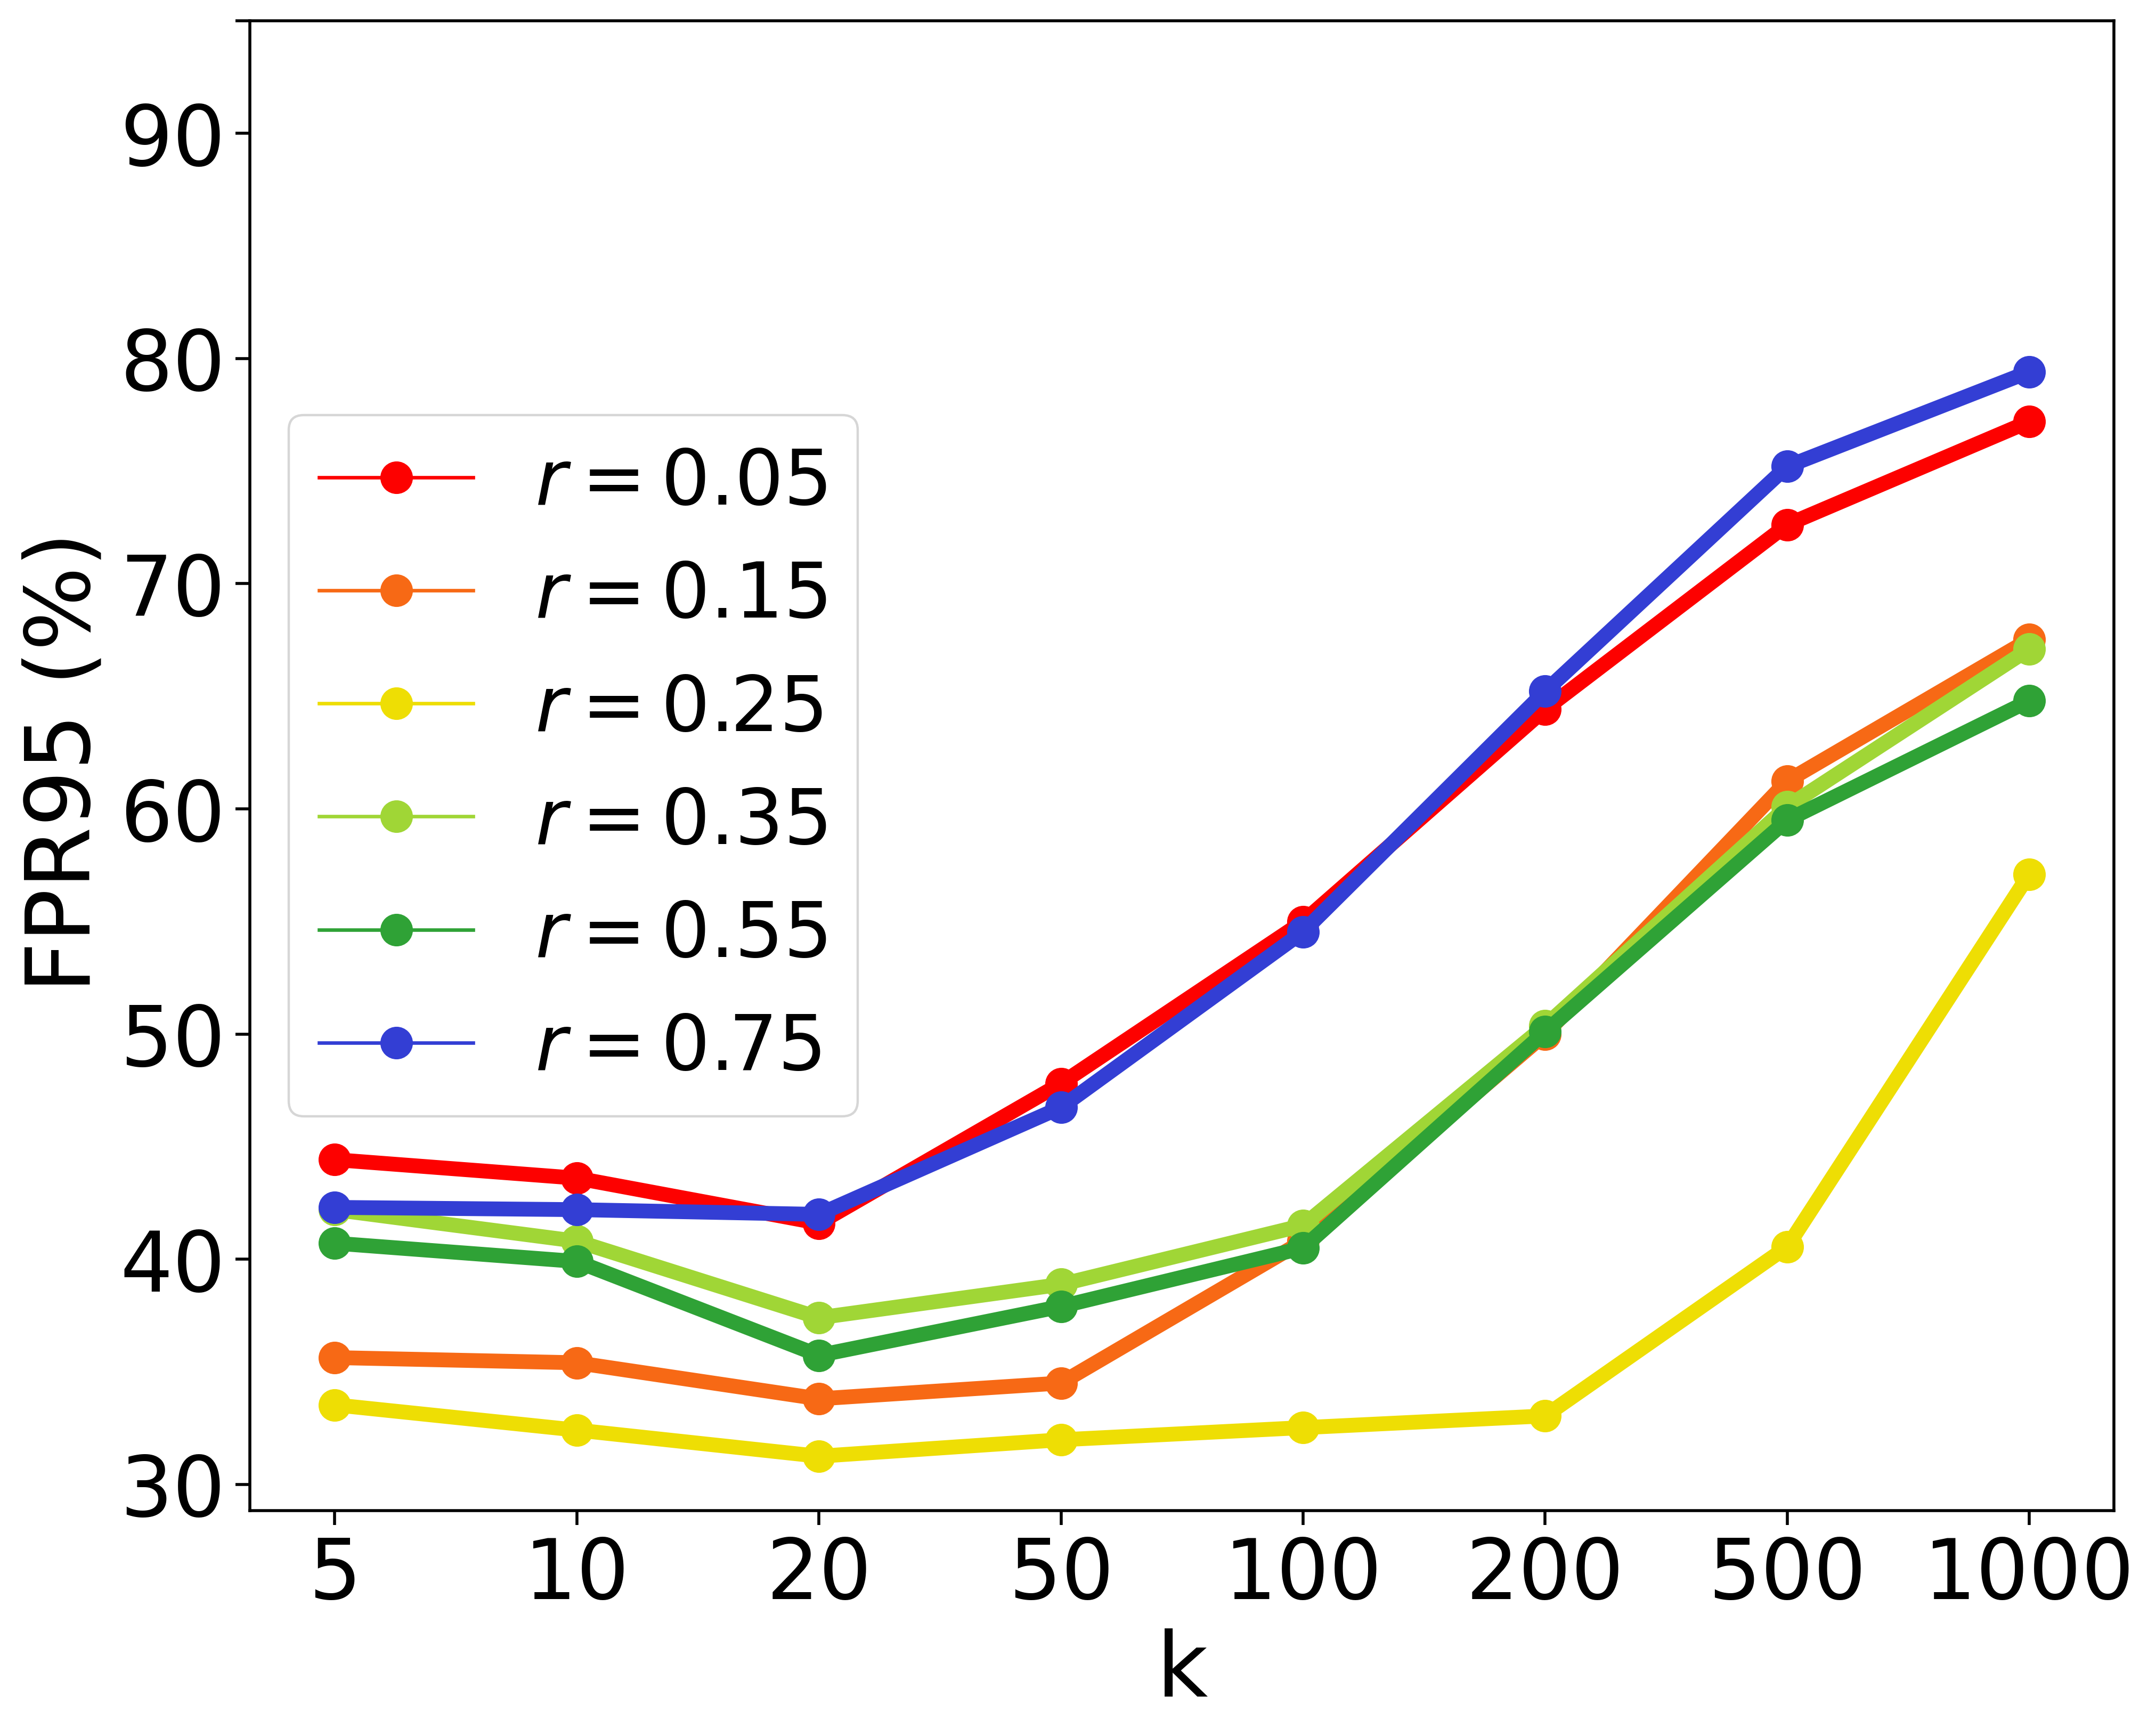
\includegraphics[width=0.90\textwidth]{images/ablations_NEW_FPR.png}
  \caption{}
  \label{fig:fpr}
\end{subfigure}%
\begin{subfigure}{0.5\textwidth}
  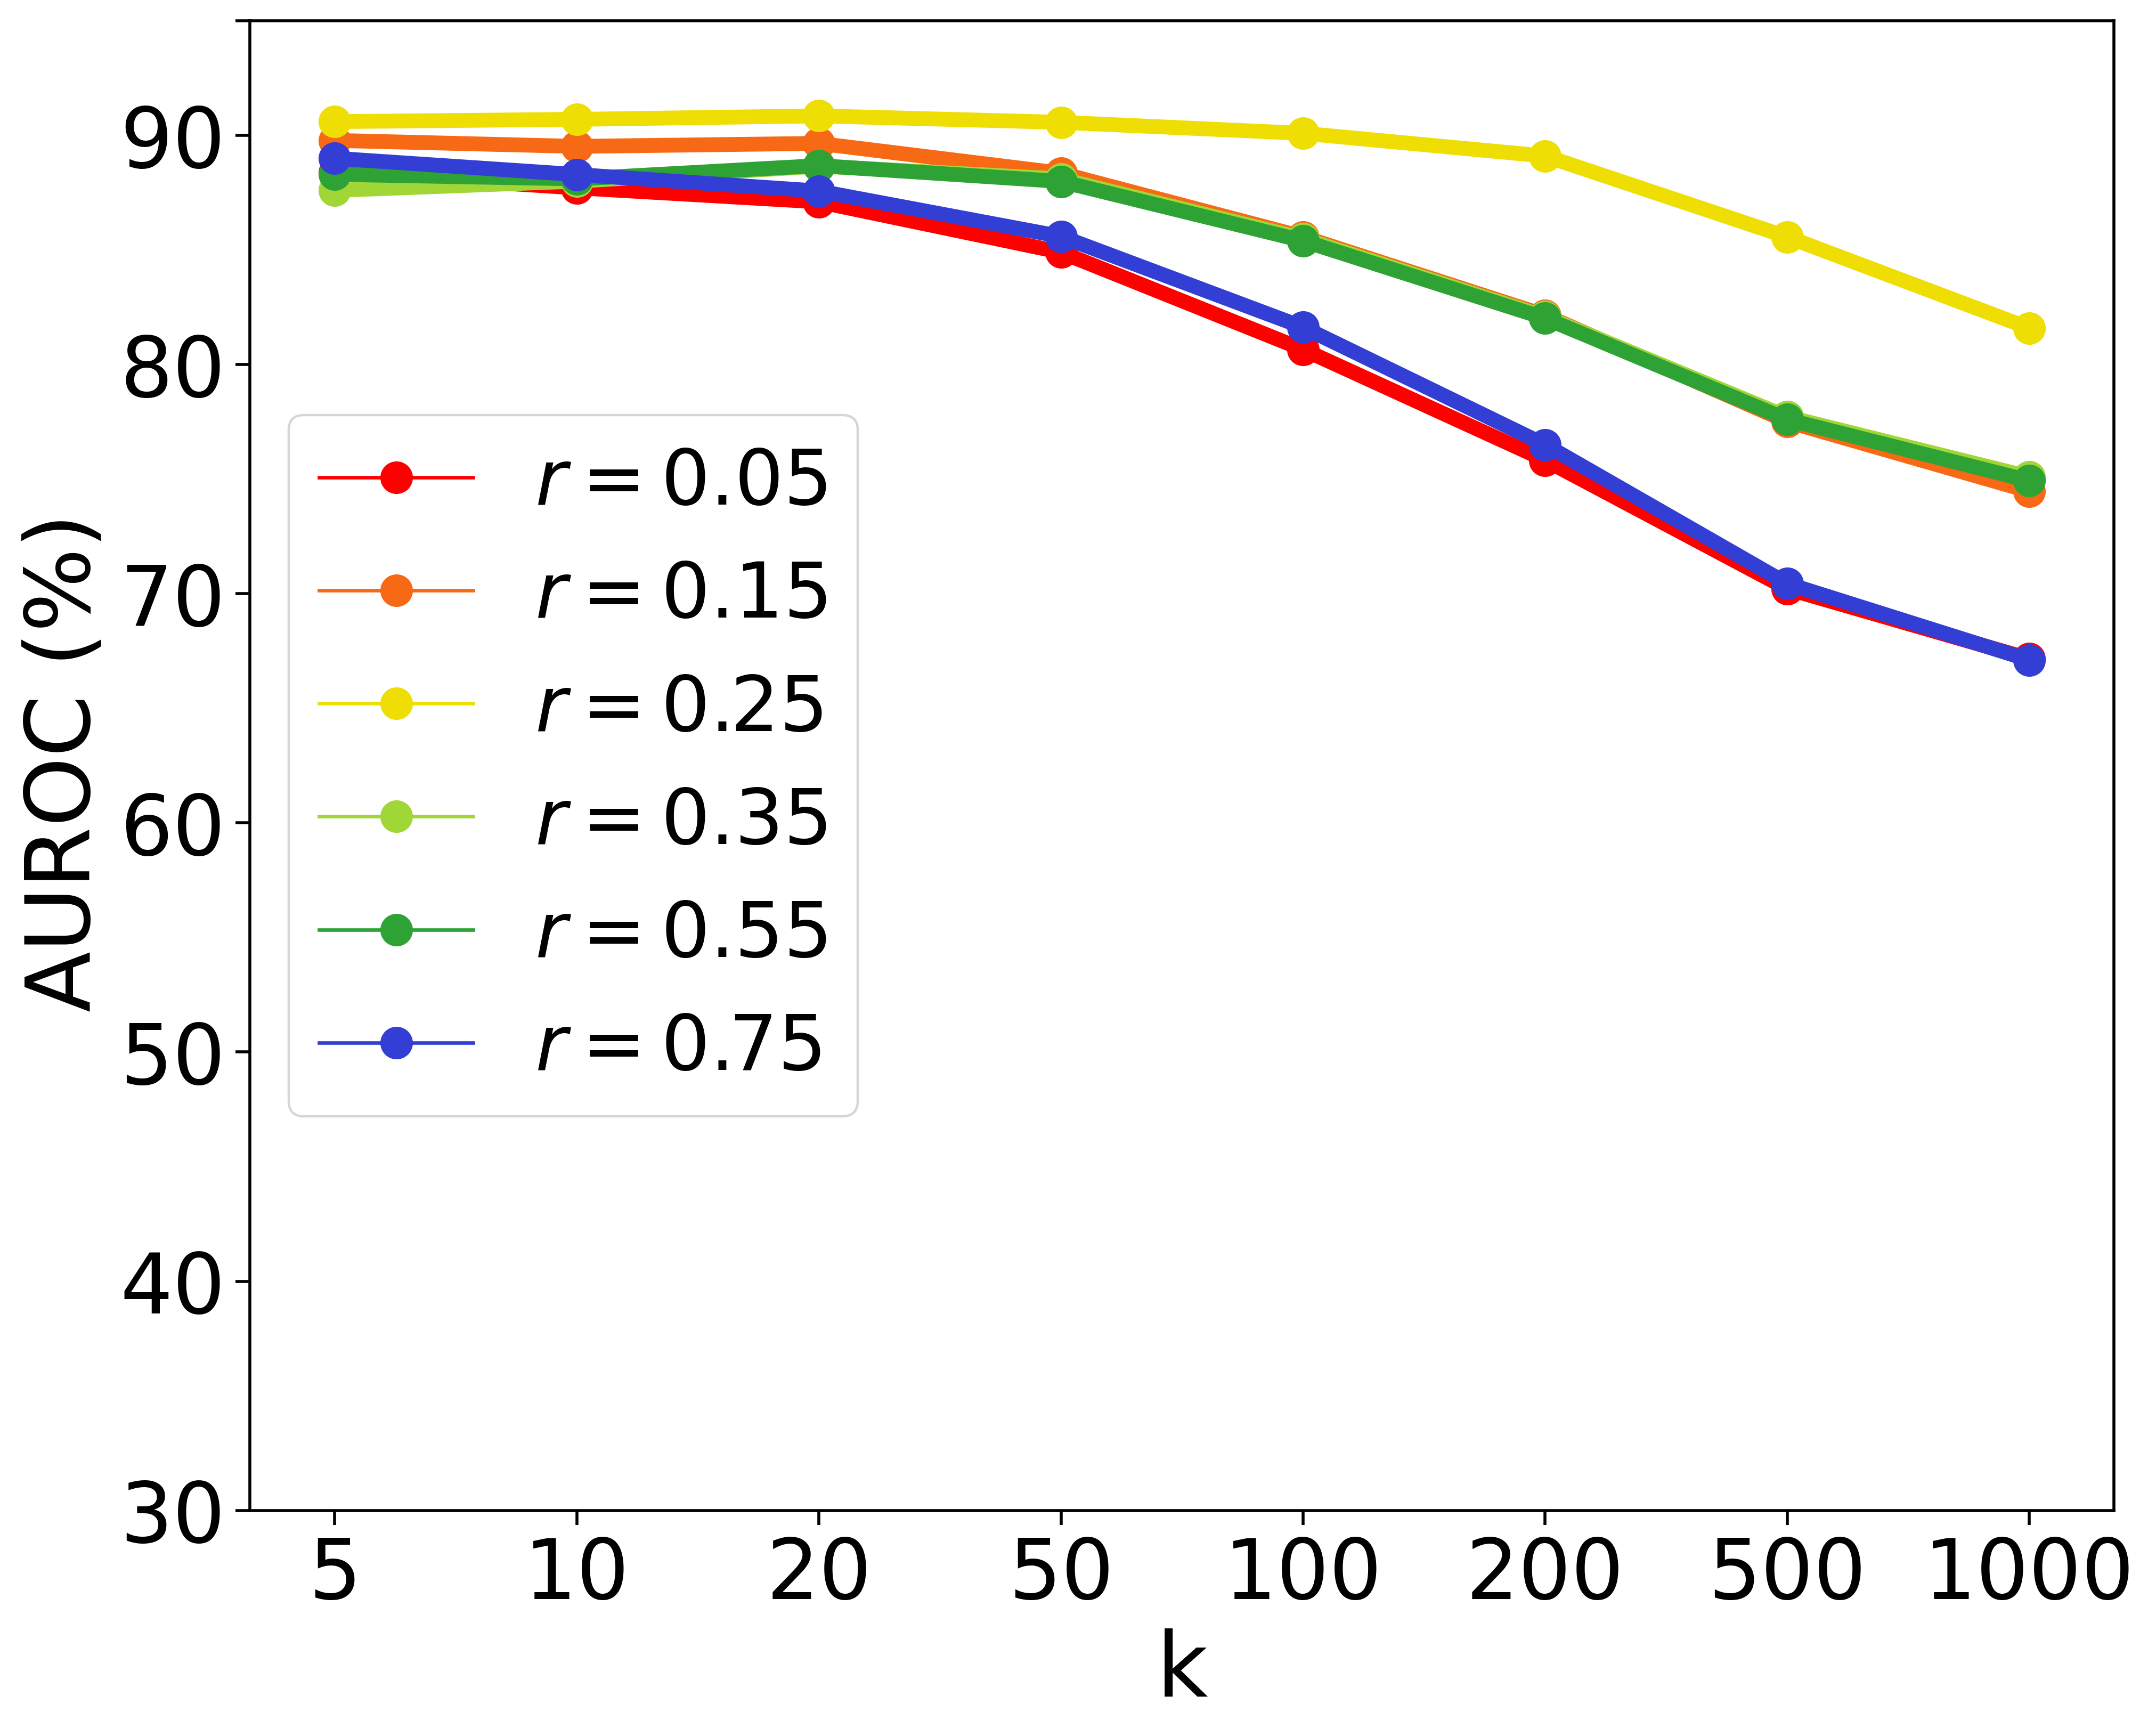
\includegraphics[width=0.90\textwidth]{images/ablations_NEW_AUROC.png}
  \caption{}
  \label{fig:auroc}
\end{subfigure}
\caption{\small Visualization of the relationship between the hyper-parameters $r$ and $k$ through OOD detection performance. The model is DenseNet-101 and ID is CIFAR-100. The OOD performance is averaged over six test datasets as mentioned in Section~\ref{sec:experiment}.}
\label{fig:relationship}
\end{figure*}

\subsection{Evaluation on Calibration}
\label{app:calibration}

\newcolumntype{?}{!{\vrule width 1pt}}
\begin{table*}[h!]
% \scriptsize
\centering
\resizebox{0.9\textwidth}{!}{%
\begin{tabular}{lcccc?cccc?cccc}
\multirow{2}{*}{\textbf{Dataset}} & \multicolumn{2}{c}{\textbf{NLL}} & \multicolumn{2}{c?}{\textbf{NLL (w. Subspace)}} & 
\multicolumn{2}{c}{\textbf{LS}} & \multicolumn{2}{c?}{\textbf{LS (w. Subspace)}} & \multicolumn{2}{c}{\textbf{FL}} & \multicolumn{2}{c}{\textbf{FL (w. Subspace)}} \\

% \multicolumn{2}{c}{\textbf{LS}} & \multicolumn{2}{c?}{\textbf{LS (w. Subspace)}}&
\cmidrule{2-13}
& SCE & ECE & SCE & ECE & SCE & ECE & SCE & ECE & SCE & ECE & SCE & ECE \\
\midrule
\multirow{1}{*}{CIFAR-10} & 11.5 & 5.6 & 9.6 &  4.4 & 8.8 & 3.9 & 8.2 & 3.8 & 6.9 & 2.3 & \textbf{3.9} & \textbf{0.8} \\
\midrule
\multirow{1}{*}{CIFAR-100} & 3.7 & 15.1 & 2.5 & 5.8  & 2.2 & 7.8 & 2.1 & \textbf{2.7} & 2.3 & 6.8 & \textbf{2.1} & 4.3 \\
% & & $\pmb{\downarrow}$ & $\pmb{\downarrow}$ & $\pmb{\downarrow}$ & $\pmb{\downarrow}$ & $\pmb{\downarrow}$ & $\pmb{\downarrow}$ & $\pmb{\downarrow}$ & $\pmb{\downarrow}$ \\  
% \multirow{1}{*}{CIFAR-10} & 11.5 & 5.6 & \cellcolor{COLOR_ZS} 9.6 & \cellcolor{COLOR_ZS} 4.4 & 8.8 & 3.9 &  \cellcolor{COLOR_ZS} 6.5 & \cellcolor{COLOR_ZS} 1.7 & 6.9 & 2.3 & \cellcolor{COLOR_ZS}\textbf{3.9} & \cellcolor{COLOR_ZS}\textbf{0.8} \\
% & ResNet-34 & 10.2 & 4.9 & \cellcolor{COLOR_ZS}9.6 & \cellcolor{COLOR_ZS}4.5 & 7.8 & 4.0 & \cellcolor{COLOR_ZS}6.3 & \cellcolor{COLOR_ZS}2.7 & 5.4 & 2.1 & \cellcolor{COLOR_ZS}\textbf{3.6} & \cellcolor{COLOR_ZS}\textbf{0.5} \\
% \midrule
% \multirow{1}{*}{CIFAR-100} & 3.7 & 15.1 & \cellcolor{COLOR_ZS}2.5 & \cellcolor{COLOR_ZS}5.8 & 2.2 & 7.8 & \cellcolor{COLOR_ZS}\textbf{2.1} & \cellcolor{COLOR_ZS}\textbf{1.9} & 2.3 & 6.8 & \cellcolor{COLOR_ZS}2.1 & \cellcolor{COLOR_ZS}4.3 \\
 % & ResNet-34 & 3.5 & 16.0 & \cellcolor{COLOR_ZS}3.5 & \cellcolor{COLOR_ZS}15.0 & 2.4 & 4.5 &\cellcolor{COLOR_ZS} \textbf{2.1} &\cellcolor{COLOR_ZS} \textbf{2.4} & 2.2 & 5.7 & \cellcolor{COLOR_ZS}2.1 & \cellcolor{COLOR_ZS}4.7 \\
%  \midrule
%  Tiny-ImageNet & ResNet-34 & 2.2 & 15.7 & \cellcolor{COLOR_ZS}1.9 & \cellcolor{COLOR_ZS}13.5 & 1.4 & 5.96 &\cellcolor{COLOR_ZS} 1.5 & \cellcolor{COLOR_ZS}3.8 & 1.4 & 2.2 & \cellcolor{COLOR_ZS}\textbf{1.3} & \cellcolor{COLOR_ZS}\textbf{1.2} \\ 
 
 
 \bottomrule

\end{tabular}%
}
\caption{\small \textbf{Calibration Results.} Comparison of calibration performance when using subspace learning with commonly used loss functions (NLL/LS/FL). The model is ResNet-50. Best performing results are marked in \textbf{bold}.}
\label{tab:calibration_1}
\end{table*}



\noindent Now we move beyond OOD detection tasks and systematically investigate the calibration performance on ID data itself. With our subspace learning, the model learns the feature subspace for each class. We hypothesize that learning the feature subspace helps alleviate the problem of over-confident predictions, thereby improving model calibration. Following the literature, we evaluate calibration performance based on two common metrics: {Expected Calibration Error (ECE)}~\cite{naeini2015obtaining} and  {Static Calibration Error (SCE)}~\cite{nixon2019measuring}. 

\paragraph{Description of calibration baselines.}

Before comparing the calibration performance, we first provide a brief description of loss functions for model calibration, along with hyperparameters in training: (1)~\textbf{Label Smoothing~\cite{muller2019does}.} In Label smoothing (LS), instead of using a one-hot encoded target $y$, a soft target vector $\*q$ is defined for each sample. Specifically, $q_i = \frac{\alpha}{C-1}$ if $i \neq y$, else $q_i = 1-\alpha, ~~~\forall i \in \{1,2,...,C\}$. Here, $\alpha$ is a hyperparameter. In this study, we set $\alpha = 0.05$. (2)~\textbf{Focal Loss~\cite{lin2017focal, mukhoti2020calibrating}.} Given input $\*x$, let $\hat{p}_c = \mathbb{P}(\hat{y}=c|\*x)$ be the output softmax probability of $\*x$ belonging to class $c$. The focal loss is defined as -$(1 - \hat{p}_y)^{\gamma}\text{log}(\hat{p}_y)$, where $y$ is the ground truth label and $\gamma$ is a user-defined hyperparameter. Following the original implementation, we set $\gamma=3$ for all experiments. 


\paragraph{Learning subspace improves calibration.} 
In Table~\ref{tab:calibration_1}, we observe that our subspace-regularized training algorithm improves calibration performance. In particular, we consider three losses that are commonly studied for calibration: (1) Cross Entropy Loss (NLL), (2) Label Smoothing~\cite{muller2019does}, and (3) Focal Loss (FL)~\cite{lin2017focal}.  We train the model with each of these losses and compare calibration performance with and without subspace regularization. For each dataset, we split the train set into two mutually exclusive sets: (1) $90\%$ of the train samples are used for training the model, and (2) the remaining $10\%$ of samples are used for validation. We observe from Table~\ref{tab:calibration_1} that \name improves the calibration performance for all loss functions.


\subsection{Detailed Results on All OOD Datasets}
\label{app:results}

In Table~\ref{tab:ablation_complete_c10} and Table~\ref{tab:ablation_complete_c100}, we report detailed results on six OOD test datasets when ID is CIFAR-10/100 respectively. The architecture used for all methods (including baselines) is DenseNet-101~\cite{huang2018densely}.





\subsection{Additional Discussion }
\label{app:add_discuss}
\paragraph{Relations to Wong \etal~\cite{wong2021leveraging}.} Wong \etal~\cite{wong2021leveraging} proposed an elastic net formulation to enforce sparsity for model interpretability. Hence, their motivation is fundamentally different from the problem we are trying to solve. Specifically, we learn a feature subspace for better ID-OOD separability, whereas Wong \etal improve the debuggability of neural nets. Given penultimate feature representations $h(\*x)$, \cite{wong2021leveraging} learns a sparse linear model $h(\*x)^{\top}\*w + w_0$ using the following optimization:
\begin{equation*}
\small  \min_{\*w}  \cfrac{1}{2N}||h(\*x)^{\top}\*w + w_0 -  y||^2_{2} - \lambda \left ( \cfrac{(1-\alpha)}{2}||\*w||_2^2 + \alpha||\*w||_1 \right),
\end{equation*}

where $\lambda$ and $\alpha$ are hyperparameters. In Table~\ref{tab:sparsification-method}, we compare the OOD performance between \name and Wong \etal. We make two concrete observations: (1) \name clearly outperforms \cite{wong2021leveraging} in terms of OOD detection performance. This result validates the effectiveness of our proposed subspace learning algorithm. (2) Model trained using ~\cite{wong2021leveraging} leads to suboptimal ID accuracy (65.89\%). In contrast, \name maintains the ID accuracy (75.59\%) along with improved OOD performance.




\begin{table*}[h!]

\centering

\resizebox{\textwidth}{!}{%
\begin{tabular}{l*{16}c}
 \multirow{2}{1.5cm}{\textbf{Methods}} & \multicolumn{12}{c}{\textbf{OOD Datasets}} & \multicolumn{2}{c}{\multirow{2}{*}{\centering\textbf{Average}}} & \multirow{2}{*}{\centering\textbf{ID Acc.}}\\

\cmidrule{2-13}

& \multicolumn{2}{c}{\textbf{SVHN}} & \multicolumn{2}{c}{\textbf{LSUN-c}} &
\multicolumn{2}{c}{\textbf{LSUN-r}} &
\multicolumn{2}{c}{\textbf{iSUN}} & \multicolumn{2}{c}{\textbf{Textures}} & \multicolumn{2}{c}{\textbf{Places365}} & &  \\

& FPR95 & AUROC & FPR95 & AUROC & FPR95 & AUROC &  FPR95 & AUROC & FPR95 & AUROC & FPR95 & AUROC & FPR95 & AUROC & \\
 & $\pmb{\downarrow}$ & $\pmb{\uparrow}$  & $\pmb{\downarrow}$ & $\pmb{\uparrow}$ & $\pmb{\downarrow}$ &  $\pmb{\uparrow}$ & $\pmb{\downarrow}$ & $\pmb{\uparrow}$ & $\pmb{\downarrow}$ & $\pmb{\uparrow}$ & $\pmb{\downarrow}$ & $\pmb{\uparrow}$ &
 $\pmb{\downarrow}$ & $\pmb{\uparrow}$ & $\pmb{\uparrow}$  \\
\midrule
\emph{Methods using Model Outputs}\\

MSP~\cite{hendrycks2016baseline} & 43.49 & 94.01 & 44.42 & 94.13 & 47.39 & 93.48 & 47.80 & 93.48 & 66.03 & 87.26 & 63.52 & 88.37 & 52.11 & 91.79 & 94.03\\
ODIN~\cite{liang2018enhancing} & 34.15 & 94.73 & 8.39 & 98.42 & 8.93 & 98.20 & 9.33 & 98.17 & 56.37 & 85.83 & 41.76 & 91.50 & 26.47 & 94.48 & 94.03 \\ 
GODIN~\cite{hsu2020generalized} & 3.78 & 99.17 & 9.47 & 97.83 & 5.40 & 98.67 & 6.73 & 98.54 & 23.90 & 94.32 & 55.24 & 86.52 & 17.42 & 95.84 & 94.22  \\
Energy Score~\cite{liu2020energy} & 33.07 & 95.01 & 8.10 & 98.43 & 14.04 & 97.47 & 14.58 & 97.42 & 59.61 & 85.42 & 41.98 & 91.48 & 28.40 & 94.22 & 94.03 \\

ReAct~\cite{sun2021react} & 43.67 & 94.27 & 22.37 & 96.22 & 16.68 & 97.09 & 19.81 & 96.74 & 53.44 & 89.63 & 43.23 & 91.88 & 33.12 & 94.32 & 93.27\\

GradNorm~\cite{huang2021importance} & 25.07 & 93.91 & 0.41 & 99.85 & 9.51 & 98.08 & 10.41 & 97.97 & 44.72 & 83.23 & 58.65 & 82.45 & 24.79 & 92.58 & 94.03 \\
LogitNorm~\cite{wei2022mitigating} & 14.31 & 97.63 & 2.61 & 99.37 & 17.16 & 97.18 & 17.14 & 97.16 & 39.66 & 91.17 & 47.30 & 90.40 & 19.61 & 95.51 & 93.94\\ 
DICE~\cite{sun2022dice} & 27.84 & 94.98 & 0.38 & 99.90 & 4.43 & 99.03 & 5.14 & 98.97 & 45.85 & 86.97 & 45.41 & 90.03 & 20.83 & 95.24 & 94.38 \\
\midrule
\emph{Methods using feature representations}\\
Mahalanobis~\cite{lee2018simple} & 17.85 & 94.66 & 68.49 & 76.21 & 30.06 & 92.16 & 29.86 & 91.15 & 30.73 & 88.83 & 90.34 & 52.37  & 44.55 & 82.56 & 94.03 \\ 

KNN~\cite{sun2022knn} & 3.87 & 99.31 & 10.81 & 98.13 & 12.58 & 97.75 & 12.24 & 97.87 & 21.61 & 96.07 & 49.36 & 89.54 & 18.50 & 96.36 & 94.03\\
\midrule
 \name (Ours) & 2.67 & 99.52 & 5.22 & 99.14 & 9.70 & 98.35 & 8.94 & 98.44 & 19.84 & 96.51 & 43.62 & 90.98 & \textbf{15.00} & \textbf{97.16} & 94.15 \\
\bottomrule

\end{tabular}}
\caption{table}{\small Detailed results on six OOD benchmark datasets: \texttt{Textures}~\cite{cimpoi2014describing}, \texttt{SVHN}~\cite{svhn}, \texttt{LSUN-Crop}~\cite{yu2015lsun}, \texttt{LSUN-Resize}~\cite{yu2015lsun}, \texttt{iSUN}~\cite{xu2015turkergaze}, and \texttt{Places365}~\cite{zhou2017places}. Model is DenseNet and ID is CIFAR-10.}
\label{tab:ablation_complete_c10}
\end{table*}
\begin{table*}[h!]
\centering
\resizebox{\textwidth}{!}{%
\begin{tabular}{l*{16}c}
 \multirow{2}{1.5cm}{\textbf{Methods}} & \multicolumn{12}{c}{\textbf{OOD Datasets}} & \multicolumn{2}{c}{\multirow{2}{*}{\centering\textbf{Average}}} & \multirow{2}{*}{\centering\textbf{ID Acc.}}\\

\cmidrule{2-13}

& \multicolumn{2}{c}{\textbf{SVHN}} & \multicolumn{2}{c}{\textbf{LSUN-c}} &
\multicolumn{2}{c}{\textbf{LSUN-r}} &
\multicolumn{2}{c}{\textbf{iSUN}} & \multicolumn{2}{c}{\textbf{Textures}} & \multicolumn{2}{c}{\textbf{Places365}} & &  \\

& FPR95 & AUROC & FPR95 & AUROC & FPR95 & AUROC &  FPR95 & AUROC & FPR95 & AUROC & FPR95 & AUROC & FPR95 & AUROC & \\
 & $\pmb{\downarrow}$ & $\pmb{\uparrow}$  & $\pmb{\downarrow}$ & $\pmb{\uparrow}$ & $\pmb{\downarrow}$ &  $\pmb{\uparrow}$ & $\pmb{\downarrow}$ & $\pmb{\uparrow}$ & $\pmb{\downarrow}$ & $\pmb{\uparrow}$ & $\pmb{\downarrow}$ & $\pmb{\uparrow}$ &
 $\pmb{\downarrow}$ & $\pmb{\uparrow}$ & $\pmb{\uparrow}$  \\
\midrule
\emph{Methods using Model Outputs}\\

MSP~\cite{hendrycks2016baseline} & 83.67 & 75.46 & 61.00 & 86.00 & 74.73 & 76.13 & 76.10 & 75.48 & 86.17 & 71.65 & 83.31 & 73.97 & 77.59 & 76.47 & 75.14 \\
ODIN~\cite{liang2018enhancing} & 91.51 & 76.16 & 15.16 & 97.41 & 31.92 & 93.93 & 36.75 & 92.89 & 83.92 & 72.70 & 79.12 & 77.13 & 56.39 & 86.02 & 75.14 \\
GODIN~\cite{hsu2020generalized} & 15.25 & 97.15 & 30.65 & 93.66 & 42.75 & 93.02 & 38.50 & 93.53 & 47.98 & 89.62 & 89.37 & 70.23 & 44.08 & 89.05 & 74.22 \\
Energy Score~\cite{liu2020energy} & 87.94 & 78.07 & 13.81 & 97.61 & 35.82 & 92.98 & 40.75 & 91.78 & 84.38 & 71.81 & 79.91 & 76.71 & 57.07 & 84.83 & 75.14\\
ReAct~\cite{sun2021react} & 93.65 & 74.20 & 52.07 & 87.63 & 63.14 & 88.13 & 69.96 & 85.56 & 87.07 & 72.56 & 87.90 & 67.66 & 75.06 & 79.51 & 66.56 \\ 
GradNorm~\cite{huang2021importance} & 60.62 & 87.76 & 0.65 & 99.78 & 82.20 & 75.48 & 78.68 & 78.14 & 65.73 & 71.99 & 90.41 & 65.65 & 63.05 & 79.80 & 75.14 \\
LogitNorm~\cite{wei2022mitigating} & 57.65 & 89.32 & 12.37 & 97.76 & 70.53 & 84.94 & 71.27 & 84.54 & 74.91 & 75.20 & 78.00  & 78.42 & 61.10 & 84.72 & 75.42 \\
DICE~\cite{sun2022dice} & 59.80 & 88.29 & 0.91 & 99.74 & 51.62 & 89.32  & 49.48 & 89.51 & 61.42 & 77.12 & 80.27 & 77.40 & 49.72 & 87.23 & 68.65 \\
\midrule
\emph{Methods using feature representations}\\
Mahalanobis~\cite{lee2018simple} & 70.19 & 80.49 & 93.98 & 66.81 & 24.83 & 94.97 & 26.20 & 94.19 & 31.76 & 90.01 & 94.60 & 55.17 & 56.93 & 80.27 & 75.14\\
KNN~\cite{sun2022knn} & 23.54 & 95.34 & 66.59 & 77.98 & 37.83 & 92.88 & 32.83 & 93.63 & 28.58 & 92.36 & 93.92 & 59.42 & 47.21 & 85.27  & 75.14 \\
\midrule
 \name (Ours) & 11.56 & 97.68 & 24.43 & 94.44 & 19.19 & 96.17 & 21.21 & 95.46 & 22.93 & 94.75 & 88.17 & 66.58 & \textbf{31.25} & \textbf{90.85} & 75.59 \\
\bottomrule

\end{tabular}}
\caption{table}{\small Detailed results on six OOD benchmark datasets: \texttt{Textures}~\cite{cimpoi2014describing}, \texttt{SVHN}~\cite{svhn}, \texttt{LSUN-Crop}~\cite{yu2015lsun}, \texttt{LSUN-Resize}~\cite{yu2015lsun}, \texttt{iSUN}~\cite{xu2015turkergaze}, and \texttt{Places365}~\cite{zhou2017places}. Model is DenseNet and ID is CIFAR-100.}
\label{tab:ablation_complete_c100}
\end{table*}
\end{document}